% ===========================================================
%  Regulación del Alquiler y Dinámica del Mercado Residencial
%  en Barcelona (2000–2025)  ·  Versión 3 — resultados v4
%  Compilar con pdfLaTeX en Overleaf (dos pasadas)
% ===========================================================
\documentclass[10pt,a4paper,twocolumn]{article}

\usepackage[utf8]{inputenc}
\usepackage[T1]{fontenc}
\usepackage[spanish,english]{babel}
\usepackage[top=2.0cm,bottom=2.0cm,left=1.6cm,right=1.6cm,columnsep=0.6cm]{geometry}
\usepackage{microtype}
\usepackage{lmodern}
\usepackage{times}
\usepackage{amsmath,amssymb,amsthm}
\usepackage{bm}
\usepackage{booktabs}
\usepackage{threeparttable}
\usepackage{multirow}
\usepackage{array}
\usepackage{siunitx}
\sisetup{group-separator={.}, group-minimum-digits=4}
\usepackage{graphicx}
\usepackage{subcaption}
\usepackage{float}
\usepackage[dvipsnames]{xcolor}
\usepackage[colorlinks=true,linkcolor=NavyBlue,
            citecolor=NavyBlue,urlcolor=NavyBlue]{hyperref}
\usepackage{natbib}
\usepackage{setspace}
\setstretch{1.05}
\usepackage{parskip}
\setlength{\parskip}{3pt}
\usepackage{titlesec}
\titlespacing*{\section}{0pt}{8pt}{4pt}
\titlespacing*{\subsection}{0pt}{6pt}{2pt}
\titlespacing*{\subsubsection}{0pt}{4pt}{2pt}
\titleformat{\section}{\normalfont\large\bfseries}{\thesection.}{0.5em}{}
\titleformat{\subsection}{\normalfont\normalsize\bfseries}{\thesubsection.}{0.4em}{}
\titleformat{\subsubsection}{\normalfont\small\bfseries\itshape}{\thesubsubsection.}{0.4em}{}
\usepackage{caption}
\captionsetup{font=small,labelfont=bf,skip=4pt}
\usepackage{fancyhdr}
\pagestyle{fancy}
\fancyhf{}
\fancyhead[L]{\small\textit{Soto, Ortiz, Delgado · Regulación del alquiler en Barcelona}}
\fancyhead[R]{\small\textit{2026}}
\fancyfoot[C]{\small\thepage}
\renewcommand{\headrulewidth}{0.4pt}
\usepackage{url}
\usepackage{enumitem}
\setlist[itemize]{itemsep=1pt,topsep=2pt}
\setlist[enumerate]{itemsep=1pt,topsep=2pt}
\newcommand{\pval}[1]{$p{=}#1$}
\newcommand{\MAPE}{\text{MAPE}}
\newcommand{\RMSE}{\text{RMSE}}

% ===========================================================
\begin{document}
\selectlanguage{spanish}

\twocolumn[{%
\begin{@twocolumnfalse}
\begin{center}
  {\LARGE\bfseries
   Regulación del Alquiler y Dinámica del Mercado\\[4pt]
   Residencial en Barcelona (2000--2025):\\[4pt]
   Panel de Datos, Clasificación con SHAP y SARIMAX\\[4pt]
   con Análisis de Intervención Multi-Ruptura}

  \vspace{8pt}
  {\large Katherine Soto \quad$\cdot$\quad Juan R.\ Ortiz \quad$\cdot$\quad Emilio Delgado}

  \vspace{3pt}
  {\normalsize La Salle -- Universitat Ramon Llull, Barcelona}\\[2pt]
  {\small \texttt{katherine.soto@students.salle.url.edu} \quad
          \texttt{juanricardo.ortiz@students.salle.url.edu} \quad
          \texttt{emilio.delgado@students.salle.url.edu}}

  \vspace{3pt}
  {\small Proyecto 2.1 · Mini-TFM · Máster en Inteligencia Artificial y Ciencia de Datos · Abril 2026}
\end{center}

\vspace{6pt}

\begin{abstract}
\noindent
Presentamos un análisis cuantitativo multimétodo del mercado de alquiler residencial de Barcelona
durante tres ciclos regulatorios sucesivos: Ley~11/2020, derogación del Tribunal Constitucional
(2022) y Ley~12/2023. Los datos provienen de Incasol -- Generalitat de Catalunya
(10~distritos, 2000Q1--2025Q3; 66~barrios, 2014Q1--2025Q3), el IPC del INE (base~2025),
el Euríbor del Banco de España y el Índice Socioeconómico Territorial de Idescat.
Empleamos cuatro módulos complementarios:
\textit{(i)}~regresión de panel con efectos fijos y términos de interacción de heterogeneidad
(\textit{within}, $N{=}2.838$, barrios $\times$ trimestres); \textit{(ii)}~clasificación supervisada con ingeniería de
características por retardos temporales y explicabilidad via valores SHAP;
\textit{(iii)}~modelos SARIMAX$(1,1,1)(1,0,1)_4$ con búsqueda en rejilla AIC/BIC,
test ARCH-LM de heterocedasticidad y análisis ITS-3 sobre 30 combinaciones
distrito$\times$métrica; y \textit{(iv)}~análisis de sensibilidad al sesgo de sustitución
hacia contratos de temporada. Con lag features, el AUC del Random Forest sube de 0.553 a
\textbf{0.684}, y la validación cruzada temporal confirma 0.684\,$\pm$\,0.083.
Los valores SHAP identifican el retardo-4 del crecimiento de contratos como señal dominante
de tensión. El ITS-3 muestra que la Ley~12/2023 contrae contratos
($\hat\beta_{D_{12}}{=}{-}1.588$, $p{=}0.007$) pero eleva el precio real
($+0.495$\,\euro/m$^2$, $p{=}0.034$), evidencia del efecto composición.
El punto de indiferencia del análisis de sustitución sitúa la tasa crítica de migración
a temporada en el $20.3$\,\% del volumen.
\end{abstract}

\vspace{4pt}
\noindent\textbf{Palabras clave:} regulación del alquiler · ITS multi-ruptura · panel efectos
fijos · SARIMAX · SHAP · ingeniería de features · zona tensionada · efecto composición · Barcelona.

\vspace{8pt}

\begin{otherlanguage}{english}
\begin{abstract}
\noindent
We present a multi-method quantitative study of Barcelona's residential rental market across
three successive regulatory cycles: Law 11/2020, a Constitutional Court ruling (2022), and
Law 12/2023. Data come from Incasol -- Generalitat de Catalunya (10~districts, 2000Q1--2025Q3;
66~neighbourhoods, 2014Q1--2025Q3), the CPI from INE (base~2025), Euribor from Banco de España,
and the Socioeconomic Territorial Index from Idescat. Four analytical modules are applied: \textit{(i)}~fixed-effects panel
regression with heterogeneous-impact interaction terms ($N{=}2{,}838$); \textit{(ii)}~supervised
classification with temporal lag features and SHAP explainability; \textit{(iii)}~SARIMAX
models with AIC/BIC grid search, ARCH-LM diagnostics and multi-break ITS-3 over 30
district$\times$metric combinations; and \textit{(iv)}~a sensitivity analysis for substitution
bias toward short-term contracts. Lag features raise the Random Forest AUC from 0.553 to
\textbf{0.684} (time-series CV: $0.684\pm0.083$). SHAP values identify the 4-quarter lag of
contract growth as the dominant predictor of market tension. The ITS-3 shows that Law 12/2023
reduces long-term contract volume ($\hat\beta{=}{-}1{,}588$, $p{=}0.007$) while raising real
prices ($+0.495$\,\euro/m$^2$, $p{=}0.034$), consistent with a composition effect driven by
selective supply withdrawal. The substitution-bias indifference point is 20.3\,\%.\\[2pt]
\textbf{Keywords:} rent control · interrupted time series · panel data · SARIMAX · SHAP · lag
features · tensioned market zone · composition effect · Barcelona.
\end{abstract}
\end{otherlanguage}

\vspace{10pt}\hrule\vspace{8pt}
\end{@twocolumnfalse}
}]

% ===========================================================
\section{Introducción}
\label{sec:intro}

La vivienda figura entre los retos socioeconómicos más apremiantes de las grandes
ciudades europeas en el segundo cuarto del siglo~XXI. Barcelona ofrece un caso de
estudio singular: en cinco años (2020--2025) ha transitado por tres regímenes
regulatorios del alquiler, generando una variación institucional exógena inusualmente
densa que facilita el análisis causal descriptivo con series largas y desagregación
geográfica fina.

\subsection*{Pregunta de investigación}

¿Tienen los tres ciclos regulatorios efectos estructurales, estadísticamente
distinguibles y geográficamente heterogéneos sobre el precio nominal, el precio real y
el volumen contractual del mercado de alquiler de Barcelona?

\subsection*{Contribuciones respecto a la literatura}

Frente a los trabajos anteriores para el caso español
\citep{garcia2018housing, bosch2021ley11}, este trabajo aporta cuatro elementos
metodológicos adicionales: \textit{(a)}~ingeniería de características temporales
(lags-1 y lags-4) que elevan sustancialmente la capacidad predictiva del clasificador
de tensión; \textit{(b)}~explicabilidad del modelo de clasificación mediante valores
SHAP con análisis de dependencia cruzada Euríbor$\times$precio real;
\textit{(c)}~un test de heterogeneidad de impacto regulatorio (modelo M5 con
interacción) que permite responder si la ley afecta de forma distinta a barrios de
renta alta y baja; y \textit{(d)}~un análisis formal de sensibilidad al sesgo de
sustitución hacia contratos de temporada que cuantifica la tasa crítica de migración
necesaria para que el efecto negativo sobre volumen sea estadísticamente nulo.

\subsection*{Estructura del artículo}

La Sección~\ref{sec:relacionados} revisa la literatura relevante.
La Sección~\ref{sec:datos} describe los datos y el pipeline.
La Sección~\ref{sec:metodos} desarrolla la metodología de los cuatro módulos.
La Sección~\ref{sec:resultados} reporta los resultados en secuencia.
La Sección~\ref{sec:discusion} discute las implicaciones.
La Sección~\ref{sec:conclusiones} cierra con conclusiones y líneas abiertas.

% ===========================================================
\section{Trabajo Relacionado}
\label{sec:relacionados}

\subsection{Efectos de la regulación del alquiler}

El debate académico sobre el control de rentas arranca en los modelos de primera
generación de \citet{arnott1995rent}, que predicen reducción de oferta y deterioro
del parque ante cualquier tope por debajo del precio de equilibrio. La evidencia
empírica más influyente procede de \citet{diamond2019rent}: usando la ampliación
del control en San Francisco como experimento natural, documentan una caída del 15\,\%
en la oferta de vivienda regulada, con reconversión del parque hacia usos alternativos
y un alza del 5--7\,\% en el segmento no regulado. \citet{sims2007rent} confirma
el efecto espejo con la desregulación de Massachusetts. En Europa, \citet{kholodilin2021rent}
analiza la \textit{Mietendeckel} de Berlín con diferencias en diferencias y detecta
contracción de oferta en el segmento regulado simultánea al alza en el no regulado,
patrón consistente con el que documentamos para Barcelona.

\subsection{Explicabilidad de modelos de ML en economía}

El uso de valores SHAP \citep{lundberg2017shap} para interpretar modelos de
\textit{ensemble} ha crecido rápidamente en aplicaciones de economía aplicada.
\citet{molnar2020interpretable} establece el marco teórico: los valores SHAP son
la única descomposición aditiva que satisface simultáneamente eficiencia, simetría
y linealidad. Su aplicación a mercados inmobiliarios es aún escasa;
\citet{antipov2020shap} los usa para valoración hedónica, pero no para análisis
de impacto regulatorio. Este trabajo aplica SHAP para separar el efecto de las
variables de inercia temporal (lags) del efecto de las variables de política
en la predicción de tensión contractual.

\subsection{Métodos de series temporales interrumpidas}

El diseño ITS de \citet{wagner2002its} es el estándar para evaluar intervenciones
de política cuando el grupo de control es inexistente o no comparable.
La especificación con tres rupturas simultáneas que empleamos extiende el diseño
de ruptura única al caso de intervenciones secuenciales, siguiendo la formulación
de \citet{cruz2019its}. Los errores HAC de \citet{newey1987hac} corrigen la
autocorrelación serial sin imponer estructura paramétrica. La selección del orden
SARIMAX por rejilla AIC sigue el protocolo de \citet{hyndman2021forecasting}.

% ===========================================================
\section{Datos y Preparación}
\label{sec:datos}

\subsection{Fuentes de datos, cobertura y variables}

El análisis integra cuatro fuentes de datos oficiales \citep{incasol2025,ine2025ipc,bde2025euribor,idescat2025ist}
que se combinan mediante \textit{merge} temporal por trimestre:

\begin{enumerate}[leftmargin=*,itemsep=2pt]
  \item \textbf{Contratos de alquiler (distritos y barrios):}
    Incasol -- Generalitat de Catalunya, disponible a través del portal estadístico
    de Habitatge:\\ \url{https://habitatge.gencat.cat/ca/dades/indicadors_estadistiques/estadistiques_de_construccio_i_mercat_immobiliari/mercat_de_lloguer/lloguers-barcelona-per-districtes-i-barris/}\\
    Dos granularidades de cobertura temporal diferenciadas:
    \begin{itemize}
      \item \textbf{Distritos:} 2000Q1--2025Q3 ($T{=}103$ trimestres, 10~distritos).
        Base del análisis de series temporales (Módulos~3 y~4) y origen
        del agregado ciudad usado en el Módulo~4.
      \item \textbf{Barrios:} 2014Q1--2025Q3 ($T{=}47$ trimestres, 66~barrios;
        7~barrios de mercado delgado excluidos por mediana inferior a 300
        contratos/trimestre). Exclusivamente empleados en el módulo de
        regresión de panel y clasificación.
    \end{itemize}
  \item \textbf{Índice de Precios al Consumidor (IPC):}
    Instituto Nacional de Estadística (INE), tabla 24078, base~2025.\\
    \url{https://www.ine.es/jaxiT3/Datos.htm?t=24078}
  \item \textbf{Euríbor a 12 meses:}
    Banco de España, Boletín Estadístico (BIE).\\
    \url{https://app.bde.es/bie_www/bie_wwwias/xml/Arranque.html?Idioma=es}
  \item \textbf{Índice Socioeconómico Territorial (barrios):}
    Institut d'Estadística de Catalunya (Idescat), datos abiertos IST.\\
    \url{https://www.idescat.cat/dades/obertes/ist/}\\
    Utilizado como proxy de nivel socioeconómico barrio-específico
    para la construcción del indicador $\mathbb{H}_d$ en el modelo M5.
\end{enumerate}

Definimos tres métricas analíticas que cubren dimensiones complementarias del mercado:
\begin{align}
  \texttt{avg\_rent\_m2}_t &= \frac{\sum_i w_{it} r_{it}}{\sum_i w_{it}}
  \label{eq:nominal}\\
  \texttt{avg\_rent\_m2\_real}_t &= \texttt{avg\_rent\_m2}_t \times \frac{100}{\text{IPC}_t^{(2025)}}
  \label{eq:real}\\
  \texttt{num\_contracts}_t &= \sum_i n_{it}
  \label{eq:vol}
\end{align}
donde $w_{it}$ es el número de contratos del submercado $i$ en el trimestre $t$. El
uso de la media ponderada en~\eqref{eq:nominal} evita el sesgo de composición de
tamaño de distrito. El precio real~\eqref{eq:real} está disponible desde 2002Q1;
los modelos que lo requieren arrancan en esa fecha.

La Figura~\ref{fig:eda_series} muestra la evolución temporal de las tres métricas.
La comparación entre nominal y real revela que el incremento del $+180$\,\% en
20~años es principalmente inflacionario: en términos reales la variación es del $+14$\,\%.

\begin{figure}[H]
  \centering
  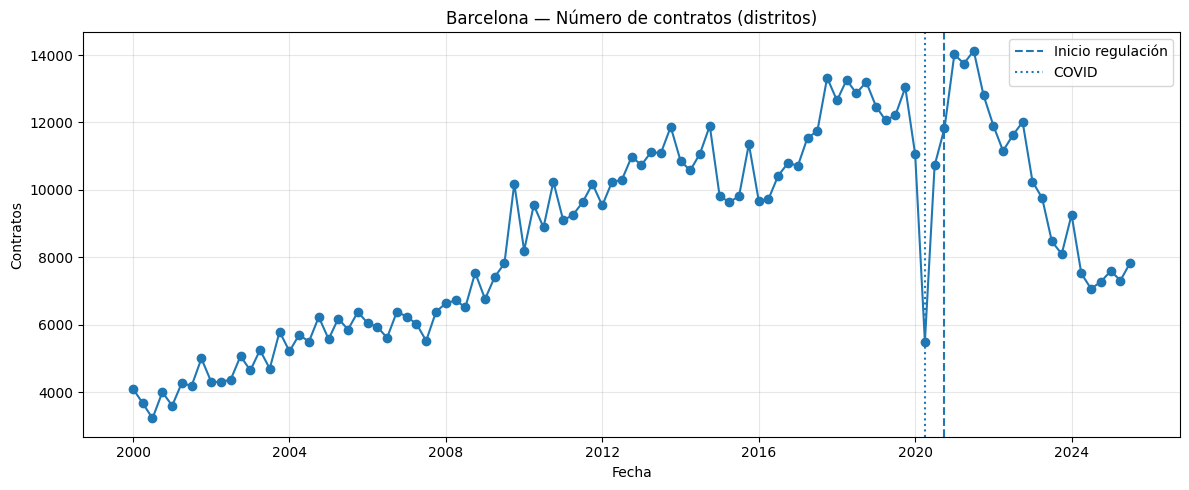
\includegraphics[width=\linewidth]{figures_v3/fig_eda_series.png}
  \caption{Series trimestrales 2000--2025 (Barcelona ciudad). Línea gris punteada:
    inicio COVID (2020Q1). Línea roja discontinua: entrada en vigor Ley 11/2020 (2020Q4).
    La divergencia entre precio nominal (subida sostenida) y precio real (plateau
    post-2021) ilustra el componente inflacionario del ciclo reciente.}
  \label{fig:eda_series}
\end{figure}

\subsection{Cambio estructural y heterogeneidad}

La Figura~\ref{fig:eda_5periods} desagrega las distribuciones por período regulatorio.
La Tabla~\ref{tab:prepost} reporta los tests formales de diferencias.

\begin{figure}[H]
  \centering
  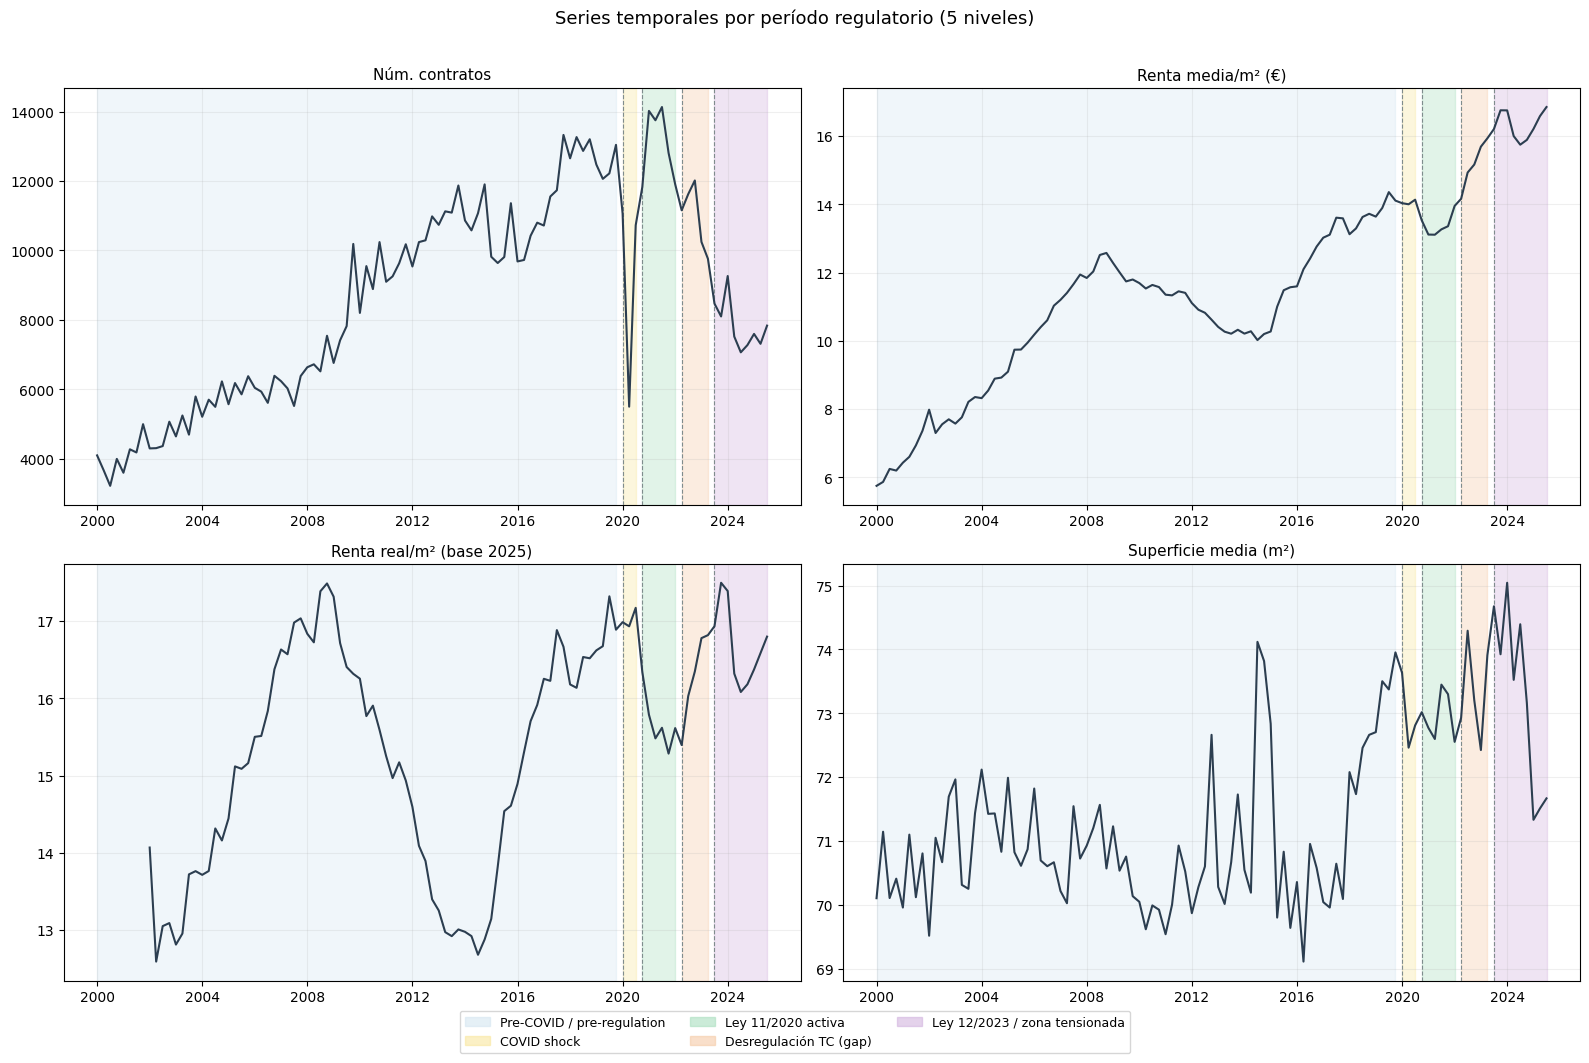
\includegraphics[width=\linewidth]{figures_v3/fig_eda_5periods.png}
  \caption{Distribución de las tres métricas por período regulatorio (2000--2025).
    P1: mercado libre; P2: COVID shock; P3: Ley~11/2020; P4: Desregulación TC;
    P5: Ley~12/2023. Los valores atípicos de P4 en precio nominal reflejan el
    ajuste de rentas en el período de vacío regulatorio.}
  \label{fig:eda_5periods}
\end{figure}

\begin{table}[H]
\caption{Tests de diferencias pre/post-regulación (Barcelona ciudad)}
\label{tab:prepost}
\centering\small
\begin{threeparttable}
\begin{tabular}{lrrl}
\toprule
Variable & $\Delta$\,M (\%) & $p$-Welch & Sig. \\
\midrule
Contratos (\texttt{n})          & $+22.9$ & $0.006$ & ** \\
Precio nominal (\euro/m$^2$)    & $+41.7$ & $<.001$ & *** \\
Precio real 2025 (\euro/m$^2$)  & $+7.2$  & $<.001$ & ** \\
Superficie (m$^2$)              & $+3.0$  & $<.001$ & *** \\
\bottomrule
\end{tabular}
\begin{tablenotes}\small
\item $n_{pre}{=}83$, $n_{post}{=}20$ obs.\ trimestrales ciudad (post = 2020Q4 en adelante).
Mann-Whitney confirma todos los resultados con $p{<}0.01$.
El $+41.7$\,\% nominal frente al $+7.2$\,\% real descompone el efecto precio en su
componente monetario (inflacionario) vs.\ ajuste real del mercado.
$^{***}p{<}.01$, $^{**}p{<}.05$.
\end{tablenotes}
\end{threeparttable}
\end{table}

El test de Chow confirma ruptura estructural en 2020Q4 para precio nominal
($F{=}5.16$, $p{=}0.007$) y contratos ($F{=}101.2$, $p{<}0.001$), pero no para
precio real ($F{=}0.28$, $p{=}0.755$). La Figura~\ref{fig:eda_chow} muestra los
estadísticos por variable.

\begin{figure}[H]
  \centering
  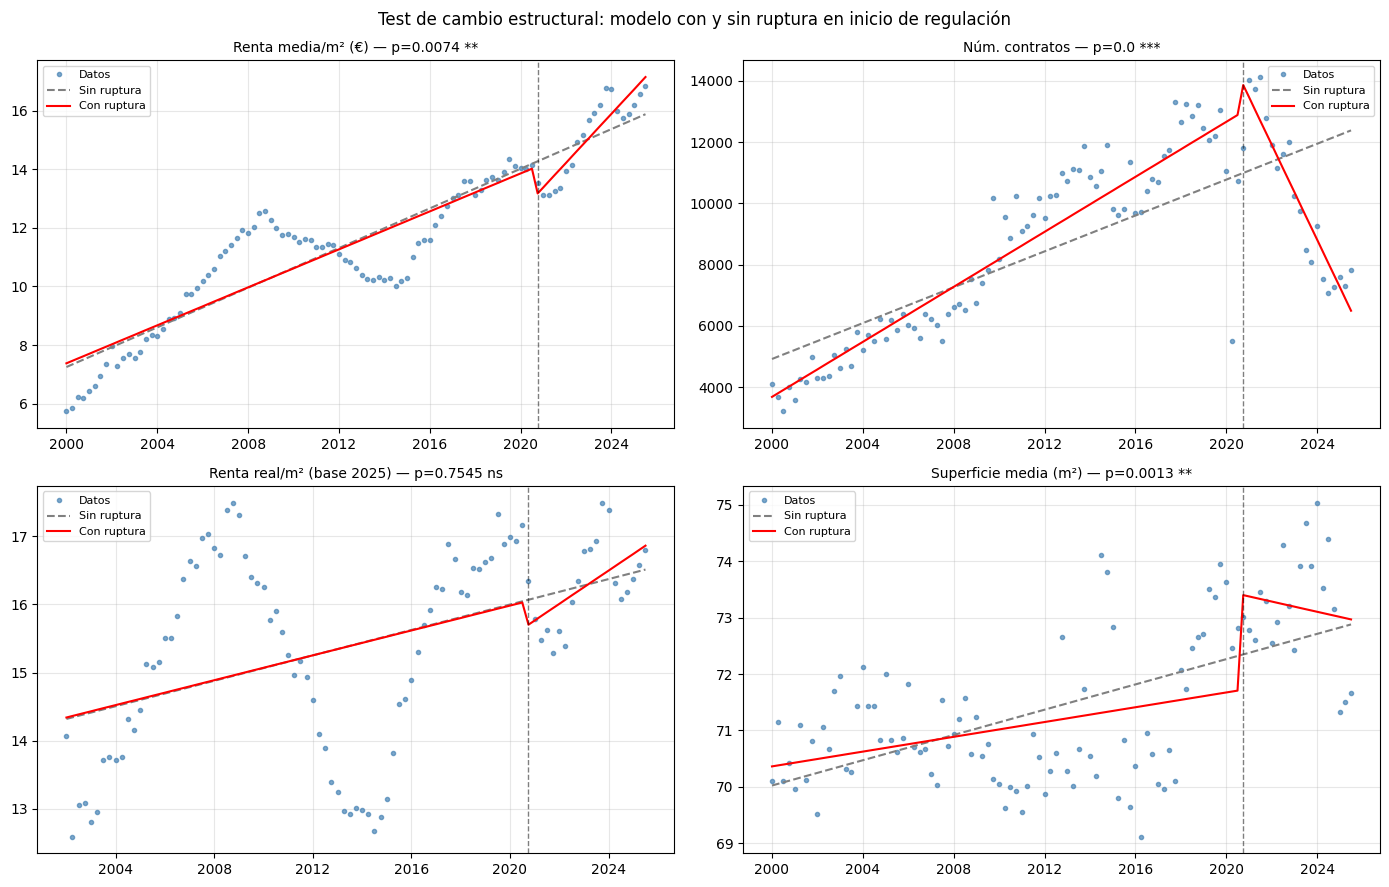
\includegraphics[width=\linewidth]{figures_v3/fig_eda_chow.png}
  \caption{Test de Chow simplificado (ruptura 2020Q4) por variable. La línea
    roja indica el umbral crítico $F_{0.05}$. El número de contratos presenta
    el estadístico más elevado ($F{>}100$), coherente con el colapso y rebote
    de 2020--2021 que domina la variación temporal de esa serie.}
  \label{fig:eda_chow}
\end{figure}

La heterogeneidad geográfica es sustancial: Sant Martí y Eixample lideran la
variación de renta real post-regulación ($+10.8$\,\% y $+10.3$\,\% respectivamente),
mientras Nou Barris prácticamente no varía ($+0.7$\,\%).

% ===========================================================
\section{Metodología}
\label{sec:metodos}

\subsection{Módulo 1 — Panel con Efectos Fijos e Interacción M5}

\subsubsection{Especificaciones M1--M3}

Estimamos el modelo \textit{within}:
\begin{equation}
  y_{it} = \alpha_i + \sum_k \beta_k z_{k,t}
         + \boldsymbol{\gamma}'\mathbf{x}_{it} + \varepsilon_{it}
  \label{eq:panel}
\end{equation}
donde $\alpha_i$ son efectos fijos barrio, $z_{k,t}$ indicadores regulatorios/macro
y $\mathbf{x}_{it}$ incluye precio, superficie y estacionalidad. El estimador es:
\begin{equation}
  \hat{\beta}_{WG}
  = \Bigl(\sum_i \ddot{\mathbf{X}}_i'\ddot{\mathbf{X}}_i\Bigr)^{-1}
    \sum_i \ddot{\mathbf{X}}_i'\ddot{y}_i, \quad
  \ddot{z}_{it} = z_{it} - \bar{z}_i
  \label{eq:within}
\end{equation}
Los errores SE se estiman con clustering por barrio \citep{baltagi2021econometric}.

\subsubsection{M5 — Heterogeneidad de impacto}

Extendemos M3 con una interacción que contrasta si el efecto regulatorio difiere
entre barrios de renta alta y baja. Definimos:
\begin{equation}
  \mathbb{H}_d = \mathbf{1}\!\left[\bar{r}_d^{(\leq 2019)} \geq
  \text{mediana}_d\right], \quad
  \text{umbral} = 14.80\;\text{\euro/m}^2_\text{real}
  \label{eq:rentaalta}
\end{equation}
y estimamos:
\begin{equation}
  y_{it} = \alpha_i + \beta_1\text{pr}_t
  + \underbrace{\beta_{1a}\,\text{pr}_t \times \mathbb{H}_{d(i)}}_{\text{interacción}}
  + \beta_2\text{cv}_{it} + \boldsymbol{\gamma}'\mathbf{x}_{it} + \varepsilon_{it}
  \label{eq:m5}
\end{equation}
El coeficiente $\beta_{1a}$ mide el diferencial de impacto entre mercados.

\subsection{Módulo 2 — Clasificación con Lag Features y SHAP}

\subsubsection{Variable objetivo}

Definimos tensión contractual como:
\begin{equation}
  \tau_{it} = \mathbf{1}\!\left[
    \text{cg}_{it} < \hat{q}_{25,i}^{(\leq 2019)} \;\wedge\;
    \text{cg}_{it} < -0.05
  \right]
  \label{eq:tension}
\end{equation}

\subsubsection{Ingeniería de características — lags}

Añadimos retardos temporales de las variables más informativas:
\begin{equation}
  x_{j,it}^{(\ell)} = x_{j,i,t-\ell}, \quad \ell \in \{1, 4\}, \quad
  j \in \{\text{cg}, r, r_{\text{real}}\}
  \label{eq:lags}
\end{equation}
Los lags-4 capturan la estacionalidad anual y el efecto de comparación interanual;
los lags-1 capturan la inercia a corto plazo. El espacio de features pasa de 10 a 16
variables. El split temporal es estricto: $\text{train}\leq 2021$, $\text{test}\geq 2022$.

\subsubsection{Valores SHAP}

Para interpretar el Random Forest usamos \texttt{TreeExplainer} \citep{lundberg2017shap},
que calcula SHAP exactos sin aproximación Monte Carlo:
\begin{equation}
  \phi_j(f, \mathbf{x}) = \sum_{S \subseteq \mathcal{F}\setminus\{j\}}
  \frac{|S|!(|\mathcal{F}|-|S|-1)!}{|\mathcal{F}|!}
  \left[f_{S\cup\{j\}}(\mathbf{x}) - f_S(\mathbf{x})\right]
  \label{eq:shap}
\end{equation}
donde $\mathcal{F}$ es el conjunto de features, $S$ un subconjunto y $f_S$ el modelo
reentrenado sobre $S$. La propiedad de eficiencia garantiza que
$\sum_{j=1}^p \phi_j = f(\mathbf{x}) - \mathbb{E}[f]$.

\subsection{Módulo 3 — SARIMAX, Búsqueda en Rejilla y Test ARCH}

\subsubsection{Selección del orden por AIC/BIC}

Antes de fijar el orden $(1,1,1)(1,0,1)_4$, realizamos una búsqueda en rejilla con
$p,q \in \{0,1,2\}$ y $P,Q \in \{0,1\}$ sobre Eixample$\times$precio nominal
(caso representativo de mayor densidad de señal):
\begin{equation}
  \text{AIC} = -2\ell(\hat{\theta}) + 2k, \qquad
  \text{BIC} = -2\ell(\hat{\theta}) + k\ln T
  \label{eq:aic}
\end{equation}

\subsubsection{SARIMAX}

Para cada par $(d,m)$ estimamos:
\begin{equation}
  \phi(B)\,\Phi(B^4)\,(1{-}B)\,y_{d,t}
  = c_d + \theta(B)\,\Theta(B^4)\,\varepsilon_{d,t} + \gamma_d\,e_t
  \label{eq:sarimax}
\end{equation}
con estimación MLE y $\texttt{cov\_type='oim'}$ \citep{harvey1989forecasting}.

\subsubsection{Test ARCH-LM}

Para verificar la homoscedasticidad de los residuos aplicamos el test ARCH de Engle:
\begin{equation}
  H_0: \alpha_1 = \cdots = \alpha_4 = 0 \quad
  \text{en} \quad \hat\varepsilon_t^2 = \gamma_0
  + \sum_{j=1}^4 \gamma_j\,\hat\varepsilon_{t-j}^2 + \nu_t
  \label{eq:arch}
\end{equation}
con estadístico $LM = T \cdot R^2_\text{aux} \xrightarrow{H_0} \chi^2(4)$.

\subsubsection{ITS-3 con errores HAC}

Especificamos tres rupturas simultáneas:
\begin{equation}
  y_t = \beta_0 + \beta_1 t
  + \sum_{k \in \mathcal{K}}\!\bigl[\beta_{2k} D_{k,t}
    + \beta_{3k} t_{k,t}^+\bigr]
  + \beta_4\text{cv}_t + \beta_5 e_t + \varepsilon_t
  \label{eq:its3}
\end{equation}
con $D_{k,t}{=}\mathbf{1}[t{\geq}t_k^*]$ y $t_{k,t}^+{=}\max(0,t{-}t_k^*)$.
Los errores HAC Newey-West con $L{=}4$ lags son:
\begin{equation}
  \hat{V}_{HAC} = (X'X)^{-1}\hat{\Omega}_{NW}(X'X)^{-1}, \quad
  \hat{\Omega}_{NW} = \sum_{l=-4}^4\!\left(1-\frac{|l|}{5}\right)\!\hat\Gamma_l
  \label{eq:hac}
\end{equation}

\subsection{Módulo 4 — Análisis de Sensibilidad: Sesgo de Sustitución}

Sea $n_t = n_t^{\text{larga}} + n_t^{\text{temp}}$ el volumen total de contratos.
El ITS-3 estima sobre $n_t^{\text{larga}}$. Si $n_t^{\text{temp}} \propto D_{ley12,t}$:
\begin{equation}
  \hat\beta_{D_{12}}^{\text{obs}} = \hat\beta_{D_{12}}^{\text{real}} - \Delta n^{\text{temp}}
  \label{eq:proxy}
\end{equation}
El \textit{punto de indiferencia} $\delta^*$ es la tasa de sustitución que anula
$\hat\beta_{D_{12}}^{\text{real}}$:
\begin{equation}
  \delta^* = \frac{-\hat\beta_{D_{12}}^{\text{obs}}}{\bar{n}_{P5}}
  \label{eq:indif}
\end{equation}
donde $\bar{n}_{P5}$ es el volumen medio observado durante el período P5.

% ===========================================================
\section{Resultados}
\label{sec:resultados}

\subsection{Panel de datos}

\subsubsection{Modelos M1--M3}

La Tabla~\ref{tab:panel} presenta los resultados.

\begin{table}[H]
\caption{Panel FE, modelos M1--M3 (dep.: $\Delta^4\log n_{it}$)}
\label{tab:panel}
\centering\small
\begin{threeparttable}
\begin{tabular}{lccc}
\toprule
 & M1 & M2 & M3 \\
\midrule
\texttt{post\_reg.}
  & $-0.015$ & $0.136^{***}$ & $0.231^{***}$ \\
  & $(-1.89)$ & $(9.96)$ & $(15.71)$ \\
\texttt{covid}
  & $0.204^{***}$ & $0.159^{***}$ & $0.040^{**}$ \\
  & $(13.4)$ & $(10.0)$ & $(2.29)$ \\
$r_{it}$ (\euro/m$^2$)
  & --- & $-0.066^{***}$ & $-0.038^{***}$ \\
  & & $(-10.8)$ & $(-4.86)$ \\
Euríbor
  & --- & --- & $-0.076^{***}$ \\
  & & & $(-7.96)$ \\
Estacional & No & No & Sí \\
\midrule
$R^2$ Within & .029 & .089 & .128 \\
Obs. & 2,838 & 2,838 & 2,838 \\
\bottomrule
\end{tabular}
\begin{tablenotes}\small
\item $t$-estadísticos entre paréntesis (SE clustered por barrio, estimador within).
$^{***}p{<}.01$, $^{**}p{<}.05$. La variable dependiente es el crecimiento interanual del
número de contratos ($\Delta^4\log n_{it}$). Todos los modelos incluyen efectos fijos por
barrio. M3 añade dummies estacionales $q_2, q_3, q_4$. La elasticidad precio-contratos
en M3 ($-0.038$) implica que una subida de 1\,\euro/m$^2$ reduce el crecimiento en 3.8
puntos porcentuales, \textit{ceteris paribus}.
\end{tablenotes}
\end{threeparttable}
\end{table}

La Figura~\ref{fig:panel_resid} muestra el diagnóstico de residuos de M3.

\begin{figure}[H]
  \centering
  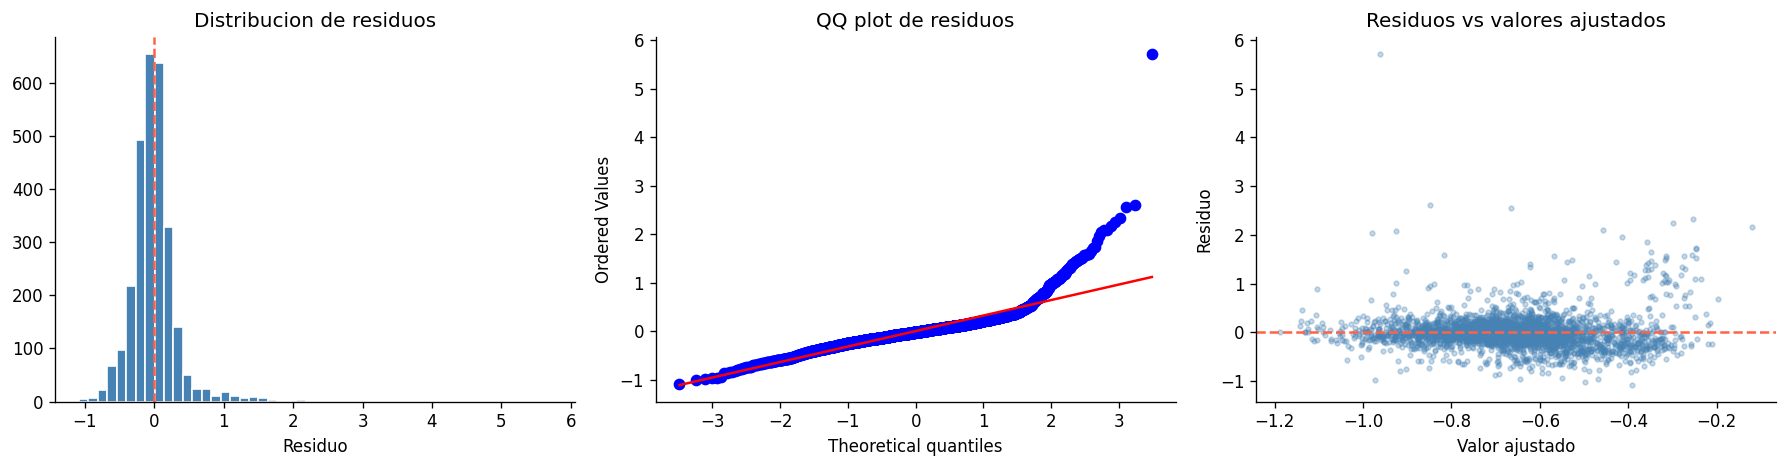
\includegraphics[width=\linewidth]{figures_v3/fig02_residuos_panel.png}
  \caption{Diagnóstico de residuos del modelo M3 (within estimator). Arriba: residuos
    vs.\ ajustados (ausencia de patrón sistemático valida la especificación); abajo:
    histograma de residuos estandarizados con asimetría moderada esperable en datos
    contractuales con cola derecha.}
  \label{fig:panel_resid}
\end{figure}

\subsubsection{M4 — Tres regímenes y M5 — Heterogeneidad de impacto}

El modelo M4 produce $\hat\delta_1{=}+0.317$ (Ley~11/2020, $p{<}.001$),
$\hat\delta_2{=}+0.001$ (derogación TC, ns) y $\hat\delta_3{=}+0.028$ (Ley~12/2023, ns).
La significancia exclusiva del primer régimen en el estimador within refleja la
dominancia del rebote post-COVID de 2020Q4.

El modelo M5 estima $\hat\beta_{1a}{=}-0.019$ ($p{=}0.301$), con efectos de
$+0.240$ en barrios de renta baja y $+0.221$ en barrios de renta alta. La diferencia
no es estadísticamente significativa, lo que indica que \textbf{el efecto regulatorio
es homogéneo entre tipos de mercado} una vez controlado el nivel de precio. La
heterogeneidad observada en el ITS-3 opera, por tanto, a través del canal de precio
(composición), no a través de una respuesta diferencial de la actividad contractual
dentro de cada barrio.

\subsection{Clasificación de tensión contractual}

\subsubsection{Impacto de los lag features}

\begin{table}[H]
\caption{Métricas de clasificación v4 con lag features (test $\geq$2022Q1)}
\label{tab:clf_v4}
\centering\small
\begin{threeparttable}
\begin{tabular}{lcccc}
\toprule
Modelo & AUC & $\Delta$AUC & AP & F1 \\
\midrule
Logística L2   & 0.627 & $+0.021$ & 0.773 & 0.765 \\
Random Forest  & \textbf{0.684} & $\mathbf{+0.131}$ & 0.760 & 0.669 \\
Grad.\ Boosting& 0.638 & $+0.065$ & 0.732 & 0.762 \\
\bottomrule
\end{tabular}
\begin{tablenotes}\small
\item $n_{train}{=}1{,}584$, $n_{test}{=}990$, $p_{+}^{test}{=}61.9$\,\%.
$\Delta$AUC = mejora respecto a la versión sin lag features (v3).
AUC-CV temporal (5 folds, RF): $0.684 \pm 0.083$.
AP = Average Precision. La mejora de $+0.131$ en el RF es sustancial: las lag features
capturan la inercia del mercado que no era observable con variables contemporáneas.
F1 reportado con umbral de clasificación 0.5.
\end{tablenotes}
\end{threeparttable}
\end{table}

La Figura~\ref{fig:roc_v4} muestra las curvas ROC y Precision-Recall.

\begin{figure}[H]
  \centering
  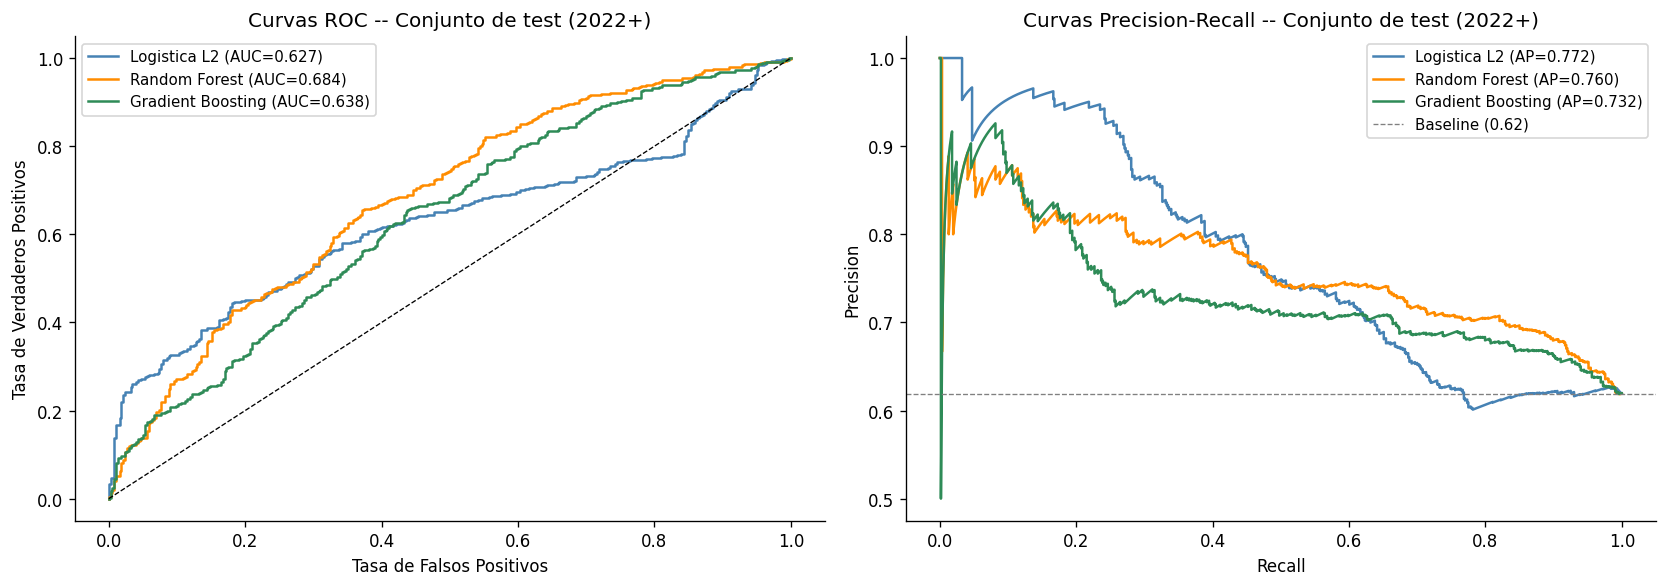
\includegraphics[width=\linewidth]{figures_v3/fig03_roc_curves.png}
  \caption{Curvas ROC (izquierda) y Precision-Recall (derecha) con lag features
    (v4). El Random Forest (azul) domina en el espacio ROC; la Regresión Logística
    mantiene mayor Average Precision en el espacio PR, lo que indica mejor
    precisión a umbrales de alta confianza. La línea punteada diagonal es el
    clasificador aleatorio (AUC = 0.5).}
  \label{fig:roc_v4}
\end{figure}

\subsubsection{Análisis SHAP}

La Figura~\ref{fig:shap_bee} muestra el beeswarm SHAP. La Tabla~\ref{tab:shap}
resume las 10 features con mayor importancia media absoluta.

\begin{figure}[H]
  \centering
  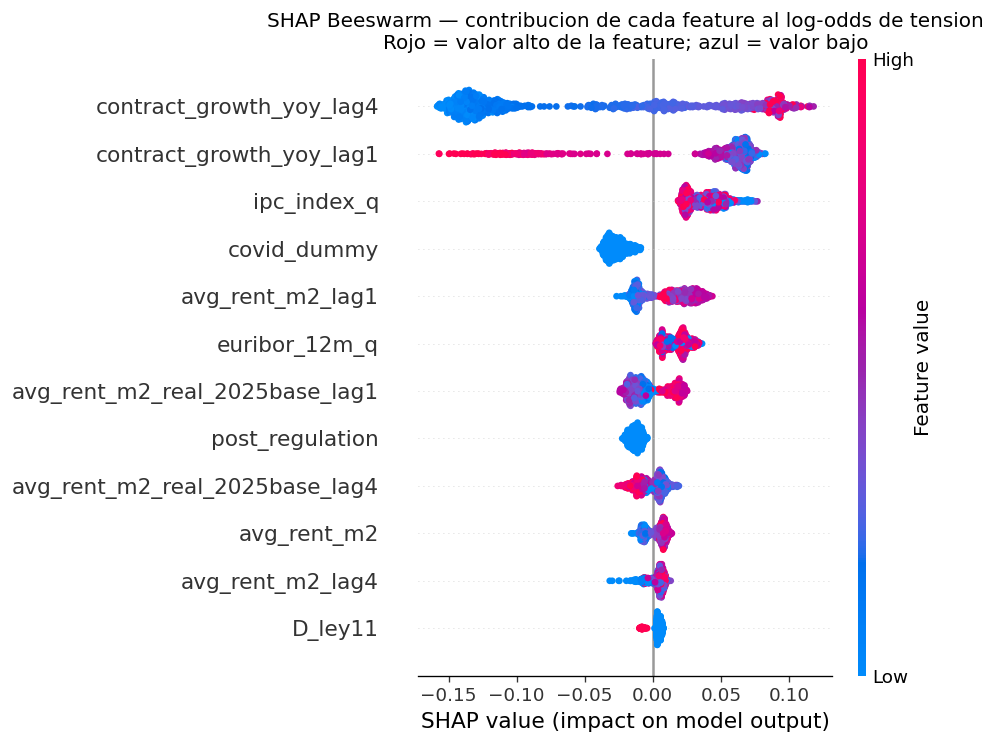
\includegraphics[width=\linewidth]{figures_v3/fig04_shap_beeswarm.png}
  \caption{Valores SHAP beeswarm (Random Forest, test 2022--2025, $n{=}990$).
    Cada punto es una observación; la posición en el eje $x$ indica la
    contribución al log-odds de tensión; el color indica el valor de la feature
    (rojo = alto, azul = bajo). La variable dominante es el retardo-4 del
    crecimiento de contratos: cuando en el mismo trimestre del año anterior
    el mercado ya mostraba caída, la probabilidad actual de tensión aumenta.}
  \label{fig:shap_bee}
\end{figure}

\begin{table}[H]
\caption{Top 10 features por importancia SHAP (media $|\phi_j|$, RF)}
\label{tab:shap}
\centering\small
\begin{threeparttable}
\begin{tabular}{lrr}
\toprule
Feature & $\overline{|\phi_j|}$ & $\bar{\phi}_j$ \\
\midrule
\texttt{contract\_growth\_lag4} & 0.0932 & $-0.047$ \\
\texttt{contract\_growth\_lag1} & 0.0662 & $+0.036$ \\
\texttt{ipc\_index\_q}          & 0.0370 & $+0.037$ \\
\texttt{covid\_dummy}           & 0.0271 & $-0.027$ \\
\texttt{avg\_rent\_m2\_lag1}    & 0.0190 & $+0.010$ \\
\texttt{euribor\_12m\_q}        & 0.0175 & $+0.018$ \\
\texttt{real\_rent\_lag1}       & 0.0130 & $-0.004$ \\
\texttt{post\_regulation}       & 0.0128 & $-0.013$ \\
\texttt{real\_rent\_lag4}       & 0.0075 & $-0.001$ \\
\texttt{avg\_rent\_m2}          & 0.0069 & $+0.003$ \\
\bottomrule
\end{tabular}
\begin{tablenotes}\small
\item $\overline{|\phi_j|}$ = importancia media absoluta (magnitud del efecto).
$\bar{\phi}_j$ = SHAP medio con signo (direccionalidad).
$\bar{\phi}_j < 0$: un valor \textit{alto} de la feature \textit{reduce} la
probabilidad de tensión; $\bar{\phi}_j > 0$: la \textit{aumenta}.
La dualidad lag4/lag1 para crecimiento de contratos (negativo/positivo) refleja
reversión a la media de primer orden: caída en $t{-}4$ predice tensión, pero
si $t{-}1$ ya mostraba recuperación, el riesgo disminuye.
\end{tablenotes}
\end{threeparttable}
\end{table}

La Figura~\ref{fig:shap_dep} muestra la dependencia parcial SHAP entre precio
real y Euríbor.

\begin{figure}[H]
  \centering
  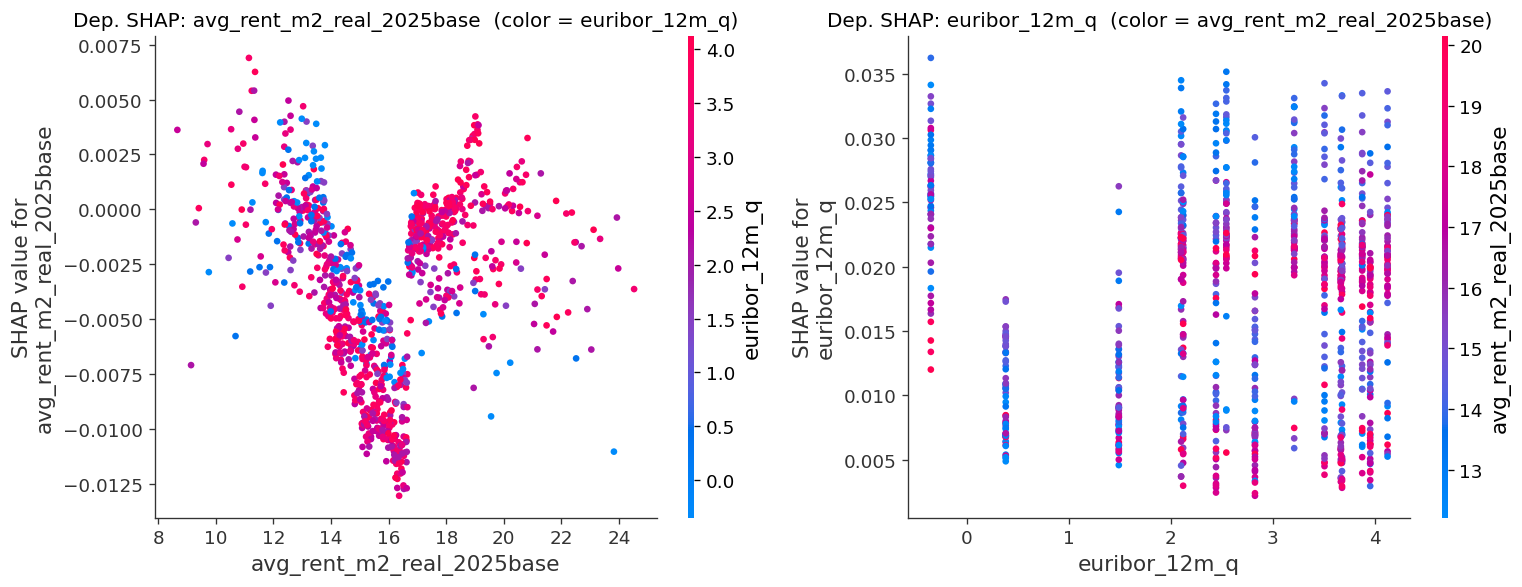
\includegraphics[width=\linewidth]{figures_v3/fig04c_shap_dependence.png}
  \caption{Dependencia parcial SHAP. Izquierda: precio real vs.\ SHAP (color =
    Euríbor); derecha: Euríbor vs.\ SHAP (color = precio real). En niveles bajos
    de precio real ($<$14\,\euro/m$^2$) el Euríbor alto amplifica la contribución
    positiva a la tensión, sugiriendo una interacción: en mercados asequibles la
    subida de tipos presiona más la demanda al no haber opción de compra.}
  \label{fig:shap_dep}
\end{figure}

\subsection{Series temporales — distrito y ciudad}

\subsubsection{Selección del orden SARIMAX}

La búsqueda en rejilla AIC sobre Eixample$\times$precio nominal muestra que el mejor
orden por AIC es $(1,1,1)(1,0,0)_4$ (AIC$=10.89$), mientras que el $(1,1,1)(1,0,1)_4$
ocupa la posición~3 (AIC$=12.82$). La diferencia es $\Delta$AIC$=1.93 < 2$, dentro
del intervalo de equivalencia estadística. Mantenemos $(1,1,1)(1,0,1)_4$ por
coherencia metodológica con el ACF/PACF (el lag-4 del MA estacional es significativo)
y porque el componente $\Theta_1$ permite capturar el error de predicción estacional
del período anterior.

\begin{figure}[H]
  \centering
  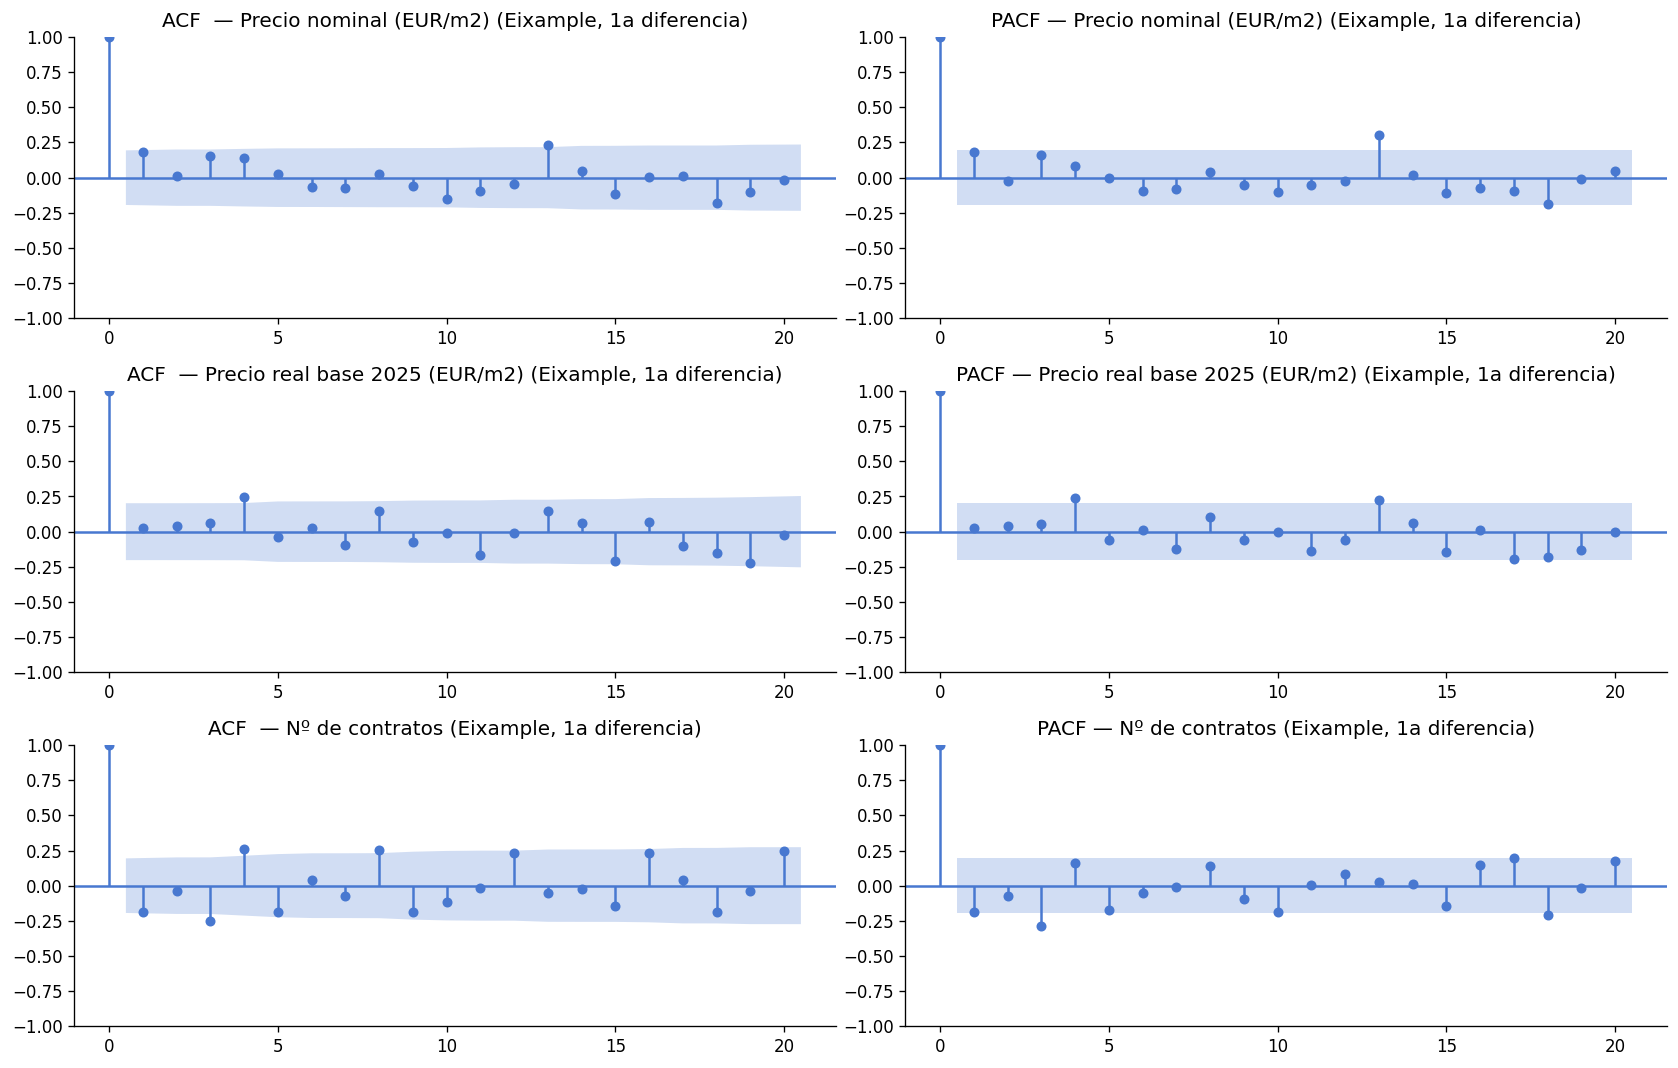
\includegraphics[width=\linewidth]{figures_v3/fig05_acf_pacf.png}
  \caption{ACF y PACF en primera diferencia para Eixample (3 métricas, filas).
    El pico significativo en lag-4 en las tres métricas confirma la necesidad del
    componente estacional $(P,D,Q)_4$. En precio real el ACF decae más lentamente,
    coherente con mayor persistencia y la clasificación I(1) ambigua en ese caso.}
  \label{fig:acf}
\end{figure}

\subsubsection{Test ARCH-LM}

De las 30 combinaciones (distrito$\times$métrica), únicamente
\textbf{Eixample$\times$\texttt{num\_contracts}} rechaza la hipótesis nula de no-ARCH
($p{=}0.0007$). El resto presenta $p > 0.05$, confirmando que los intervalos de
confianza del SARIMAX son estadísticamente válidos para precio nominal y precio real
en todos los distritos. Para la serie de contratos de Eixample, los intervalos de
confianza predictivos pueden estar subestimados y se recomienda un GARCH(1,1) si se
requiere inferencia precisa en ese caso concreto.

\subsubsection{Diagnóstico de residuos SARIMAX}

La Figura~\ref{fig:diag} muestra los paneles de diagnóstico para Eixample$\times$precio
nominal (representativo). Ljung-Box $p(\text{lag8}){=}0.985$; sin evidencia de
autocorrelación residual. El gráfico Q-Q muestra colas ligeramente pesadas, habitual
en series de precios con shocks de baja frecuencia.

\begin{figure}[H]
  \centering
  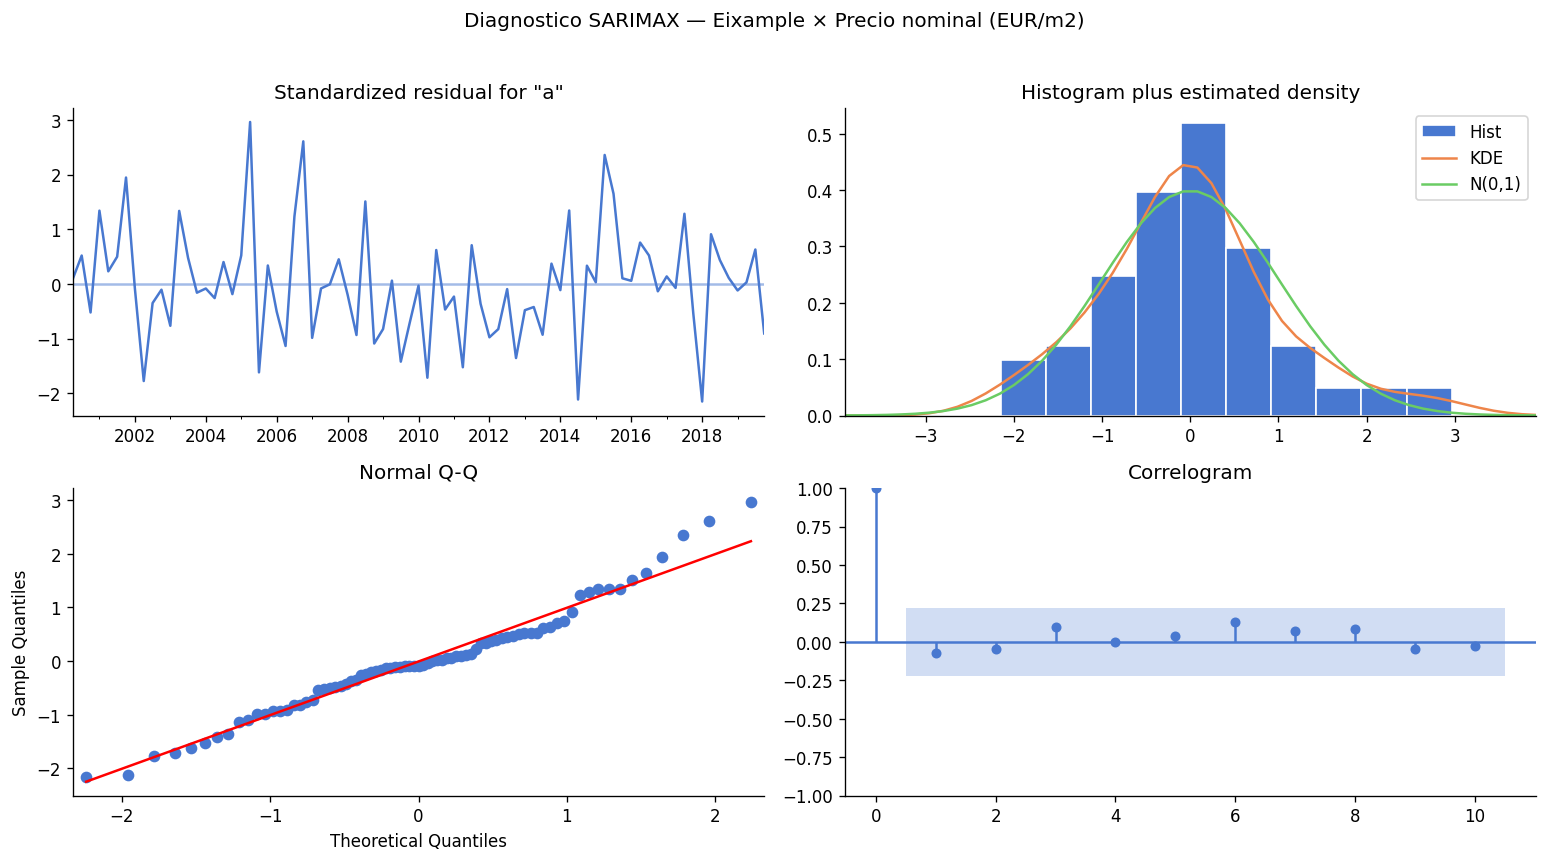
\includegraphics[width=\linewidth]{figures_v3/fig09_diagnostics_sarimax.png}
  \caption{Diagnóstico SARIMAX, Eixample$\times$precio nominal. Los cuatro paneles
    verifican: residuos sin estructura temporal, distribución aproximadamente normal
    (ligeras colas pesadas aceptables), Q-Q con leve desviación en los extremos, y
    correlograma sin picos significativos. Ljung-Box $p(8){=}0.985$ confirma ruido
    blanco en los residuos.}
  \label{fig:diag}
\end{figure}

\subsubsection{Comparativa de modelos}

\begin{table}[H]
\caption{MAPE (\%) por modelo y métrica (ciudad, test 2022Q1+)}
\label{tab:ciudad_comp}
\centering\small
\begin{threeparttable}
\begin{tabular}{lrrrl}
\toprule
Métrica & Naïve & ETS & SARIMAX & Ganador \\
\midrule
Precio nominal (\euro/m$^2$)   & 6.97 & 6.08 & \textbf{3.29} & SAR \\
Precio real 2025 (\euro/m$^2$) & 4.67 & \textbf{4.45} & 6.01 & ETS \\
N.º contratos                  & \textbf{19.43} & 51.53 & 56.83 & Naïve \\
\bottomrule
\end{tabular}
\begin{tablenotes}\small
\item SARIMAX nominal: AIC$=12.1$, BIC$=28.7$, Ljung-Box $p(8){=}0.985$.
El naïve estacional domina en contratos porque la dinámica de volumen es
principalmente estacional y el Euríbor no añade información predictiva sobre las
decisiones de firma en este horizonte. En precio nominal el SARIMAX aprovecha la
correlación temporal del Euríbor para anticipar el nivel de renta.
\end{tablenotes}
\end{threeparttable}
\end{table}

La Figura~\ref{fig:sarimax_city} compara las predicciones SARIMAX y ETS con la serie
observada bajo las bandas de períodos regulatorios.

\begin{figure}[H]
  \centering
  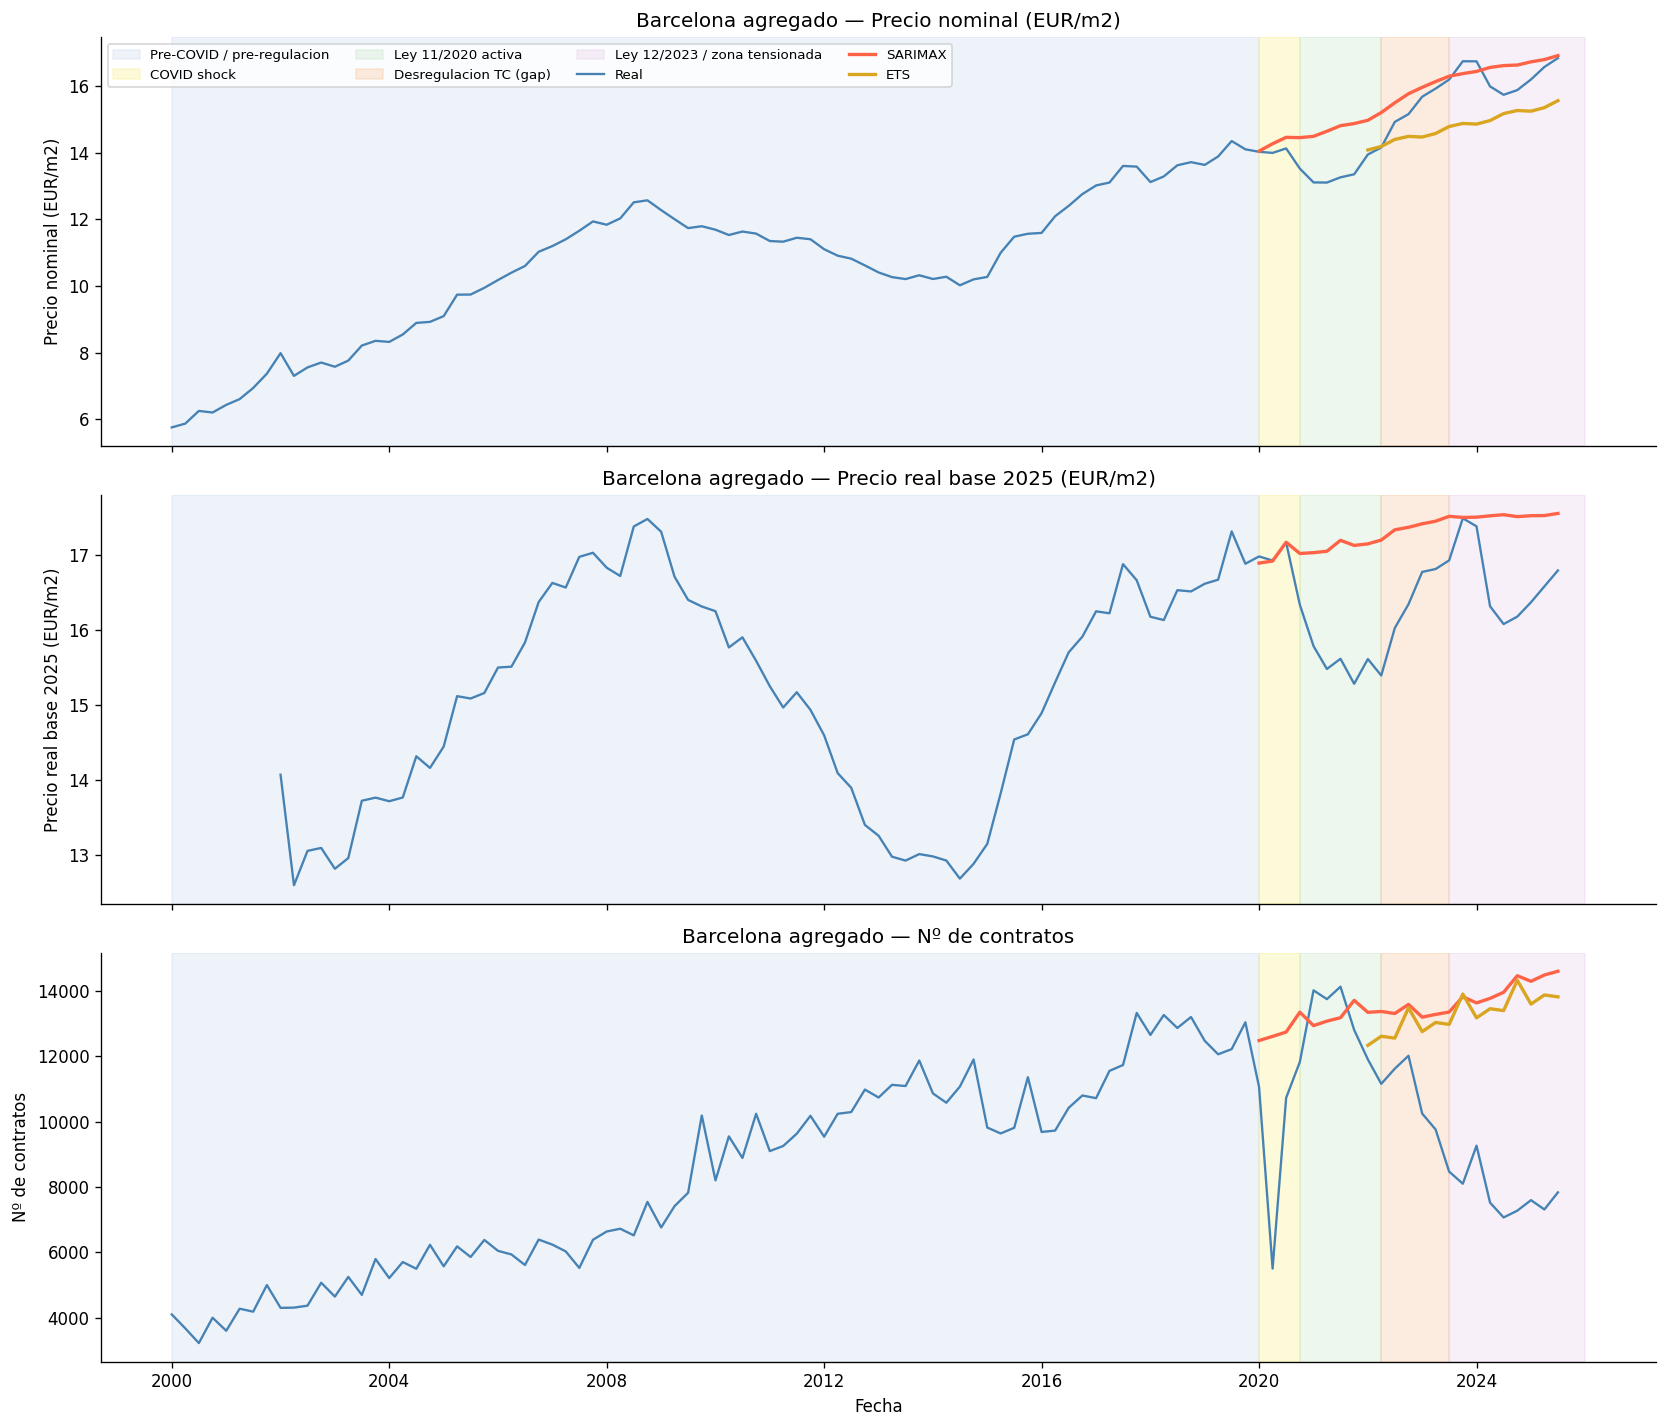
\includegraphics[width=\linewidth]{figures_v3/fig06_sarimax_city.png}
  \caption{Predicciones out-of-sample ciudad (3 métricas, 2020--2025). Línea azul:
    serie observada; rojo: SARIMAX (test desde 2020Q1); amarillo: ETS (test desde
    2022Q1). Las bandas de color identifican los cinco períodos regulatorios.
    El SARIMAX infraestima consistentemente los valores de 2024--2025, lo que
    sugiere un cambio estructural post-2023 no capturado por la dinámica ARIMA
    ni por el Euríbor.}
  \label{fig:sarimax_city}
\end{figure}

\subsubsection{ITS-3 — análisis de intervención}

La Tabla~\ref{tab:its3} reporta los coeficientes completos del ITS-3.

% ITS-3: tabla a ancho completo (table*) para evitar solapamiento en 2 columnas
\begin{table*}[ht]
\caption{ITS-3 ciudad: \textit{level shifts} y cambios de pendiente sobre las tres métricas
  (errores HAC Newey-West, $L{=}4$ lags, $T{=}103$ obs.\ trimestrales)}
\label{tab:its3}
\centering\small
\begin{threeparttable}
\begin{tabular}{l
    S[table-format=-1.3]  c
    S[table-format=-1.3]  c
    S[table-format=-4.0]  c}
\toprule
 & \multicolumn{2}{c}{\textbf{Precio nominal} (\euro/m$^2$)}
 & \multicolumn{2}{c}{\textbf{Precio real 2025} (\euro/m$^2$)}
 & \multicolumn{2}{c}{\textbf{N.º contratos/trim.}} \\
\cmidrule(lr){2-3}\cmidrule(lr){4-5}\cmidrule(lr){6-7}
\textbf{Coeficiente}
  & {$\hat{\beta}$} & {$p$\,valor}
  & {$\hat{\beta}$} & {$p$\,valor}
  & {$\hat{\beta}$} & {$p$\,valor} \\
\midrule
$D_{ley11}$\;(\textit{level shift} Ley\,11/2020)
  & -1.112 & $.007^{**}$    & -0.041 & $.942$         & -233  & $.734$        \\
$t^{+}_{ley11}$\;(pendiente post Ley\,11/2020)
  & -0.049 & $.381$         & -0.235 & $<.001^{***}$  & -179  & $.403$        \\
$D_{tc}$\;(\textit{level shift} derogación TC)
  & -0.037 & $.881$         & -0.558 & $.003^{**}$    & -681  & $.345$        \\
$t^{+}_{tc}$\;(pendiente post derogación TC)
  & -0.232 & $.134$         & -0.299 & $.021^{**}$    & -64   & $.837$        \\
$D_{ley12}$\;(\textit{level shift} Ley\,12/2023)
  & +0.383 & $.102^{\dag}$  & +0.495 & $.034^{*}$     & -1588 & $.007^{**}$   \\
$t^{+}_{ley12}$\;(pendiente post Ley\,12/2023)
  & +0.360 & $.068^{\dag}$  & +0.630 & $<.001^{***}$  & -89   & $.627$        \\
Euríbor\,12m
  & +0.654 & $<.001^{***}$  & +0.911 & $<.001^{***}$  & -307  & $<.001^{***}$ \\
\midrule
$R^2$ & \multicolumn{2}{c}{.904} & \multicolumn{2}{c}{.513} & \multicolumn{2}{c}{.918} \\
\bottomrule
\end{tabular}
\begin{tablenotes}\small
\item \textit{Nota:} HAC Newey-West con $L{=}4$ lags corrige autocorrelación serial sin imponer
estructura paramétrica. $D_k {=} \mathbf{1}[t{\geq}t_k^*]$ es el escalón de la ruptura $k$
(mide el cambio de nivel inmediato en \euro/m$^2$ para precios o en contratos/trimestre
para volumen). $t^+_k {=} \max(0,\,t - t_k^*)$ es la rampa post-ruptura (mide el cambio
de pendiente trimestral). $R^2{=}0.904$ en precio nominal indica que la tendencia lineal
+ tres rupturas explican el 90.4\,\% de la variación temporal de esa serie; $R^2{=}0.513$
en precio real refleja la mayor volatilidad de la métrica deflactada.
$^{***}p{<}.01$; $^{**}p{<}.05$; $^{*}p{<}.10$; $^{\dag}p{<}.15$.
\end{tablenotes}
\end{threeparttable}
\end{table*}

Las Figuras~\ref{fig:its3_city} y~\ref{fig:its3_dist} muestran los ajustes del
ITS-3 a nivel ciudad y por distrito, respectivamente.

\begin{figure}[H]
  \centering
  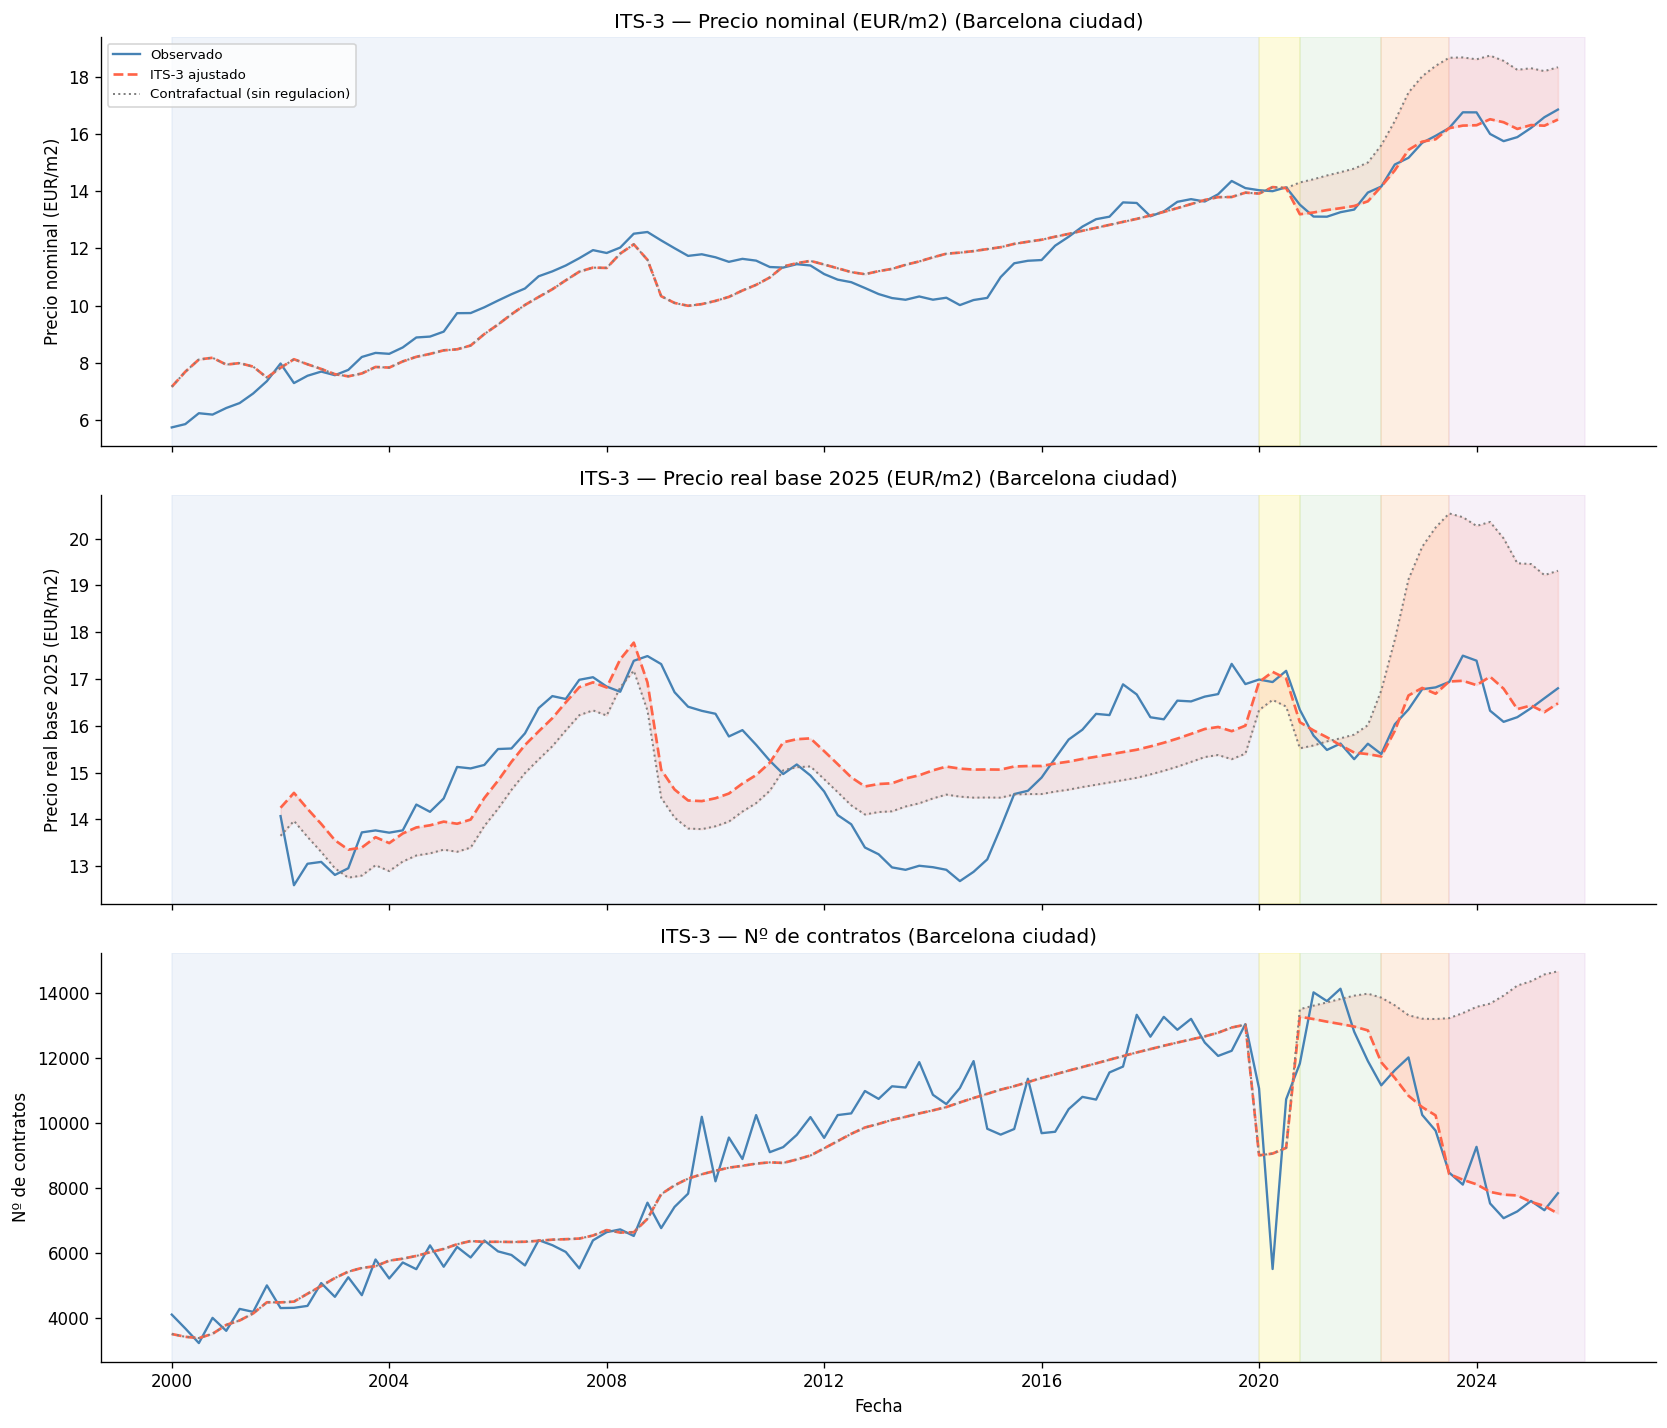
\includegraphics[width=\linewidth]{figures_v3/fig07_its3_city.png}
  \caption{ITS-3 ciudad (3 métricas). Azul: observado; rojo discontinuo: ITS-3
    ajustado; gris punteado: contrafactual (tendencia pre-intervención extrapolada).
    La brecha entre observado y contrafactual a partir de 2020Q4 acumula el efecto
    total de los tres ciclos regulatorios. La contracción de contratos post-2023Q3
    es la ruptura más limpia visualmente; el efecto sobre precio real en esa misma
    fecha es positivo, ilustrando la paradoja precio-volumen.}
  \label{fig:its3_city}
\end{figure}

\begin{figure}[H]
  \centering
  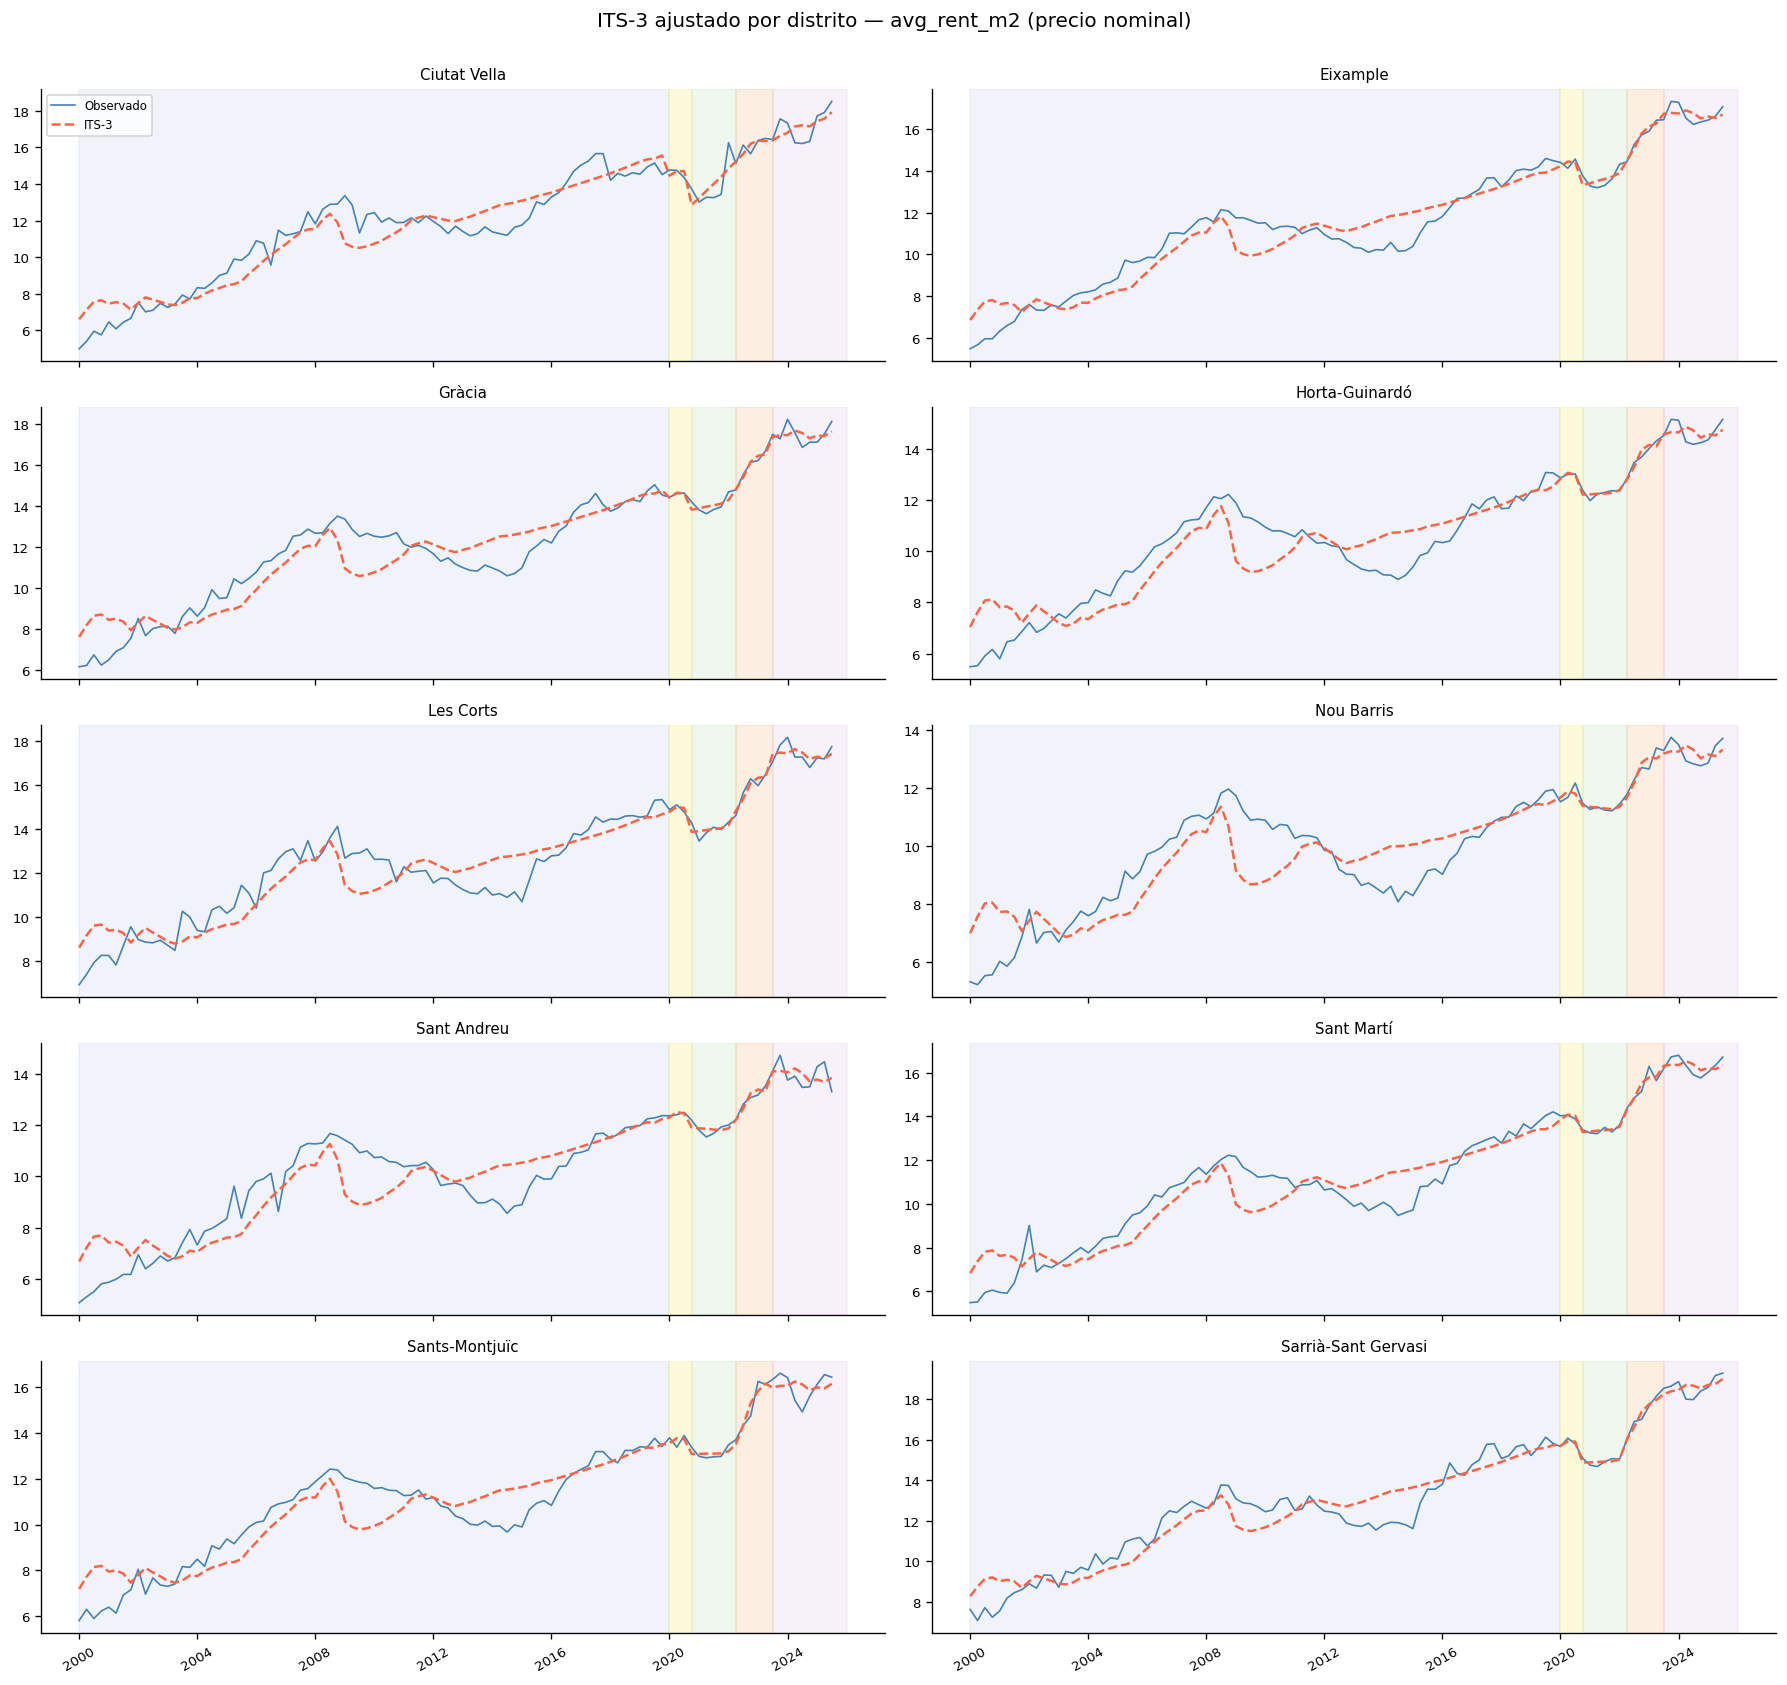
\includegraphics[width=\linewidth]{figures_v3/fig10_its3_districts.png}
  \caption{ITS-3 ajustado por distrito, precio nominal (v4). Rojo: ITS-3; azul:
    observado; bandas de color: períodos regulatorios. La brecha observado-contrafactual
    es hasta 3$\times$ mayor en Gràcia y Eixample que en Nou Barris y Horta-Guinardó,
    evidenciando la heterogeneidad geográfica del efecto regulatorio.}
  \label{fig:its3_dist}
\end{figure}

\subsubsection{Heterogeneidad geográfica del level shift $D_{ley12}$}

La Figura~\ref{fig:heatmap} muestra el heatmap del coeficiente $\hat\beta_{D_{ley12}}$
por distrito y métrica.

\begin{figure}[H]
  \centering
  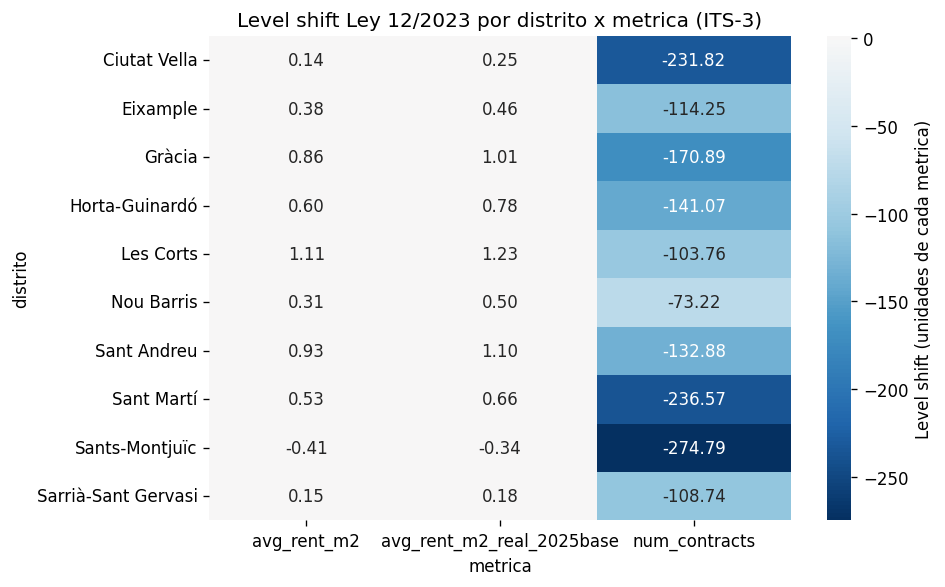
\includegraphics[width=0.92\linewidth]{figures_v3/fig10b_its3_heatmap.png}
  \caption{Level shift $\hat\beta_{D_{ley12}}$ (ITS-3) por distrito$\times$métrica.
    Rojo: efecto positivo sobre precio; azul: contracción de contratos. La divergencia
    precio-volumen es consistente en todos los distritos, confirmando que el efecto
    composición no es un artefacto de la serie agregada sino un patrón geográficamente
    robusto. Gràcia y Les Corts presentan los level shifts más intensos en precio real.}
  \label{fig:heatmap}
\end{figure}

\subsubsection{Proyecciones condicionales}

La Figura~\ref{fig:proj} muestra las proyecciones a 8 trimestres bajo dos escenarios.

\begin{figure}[H]
  \centering
  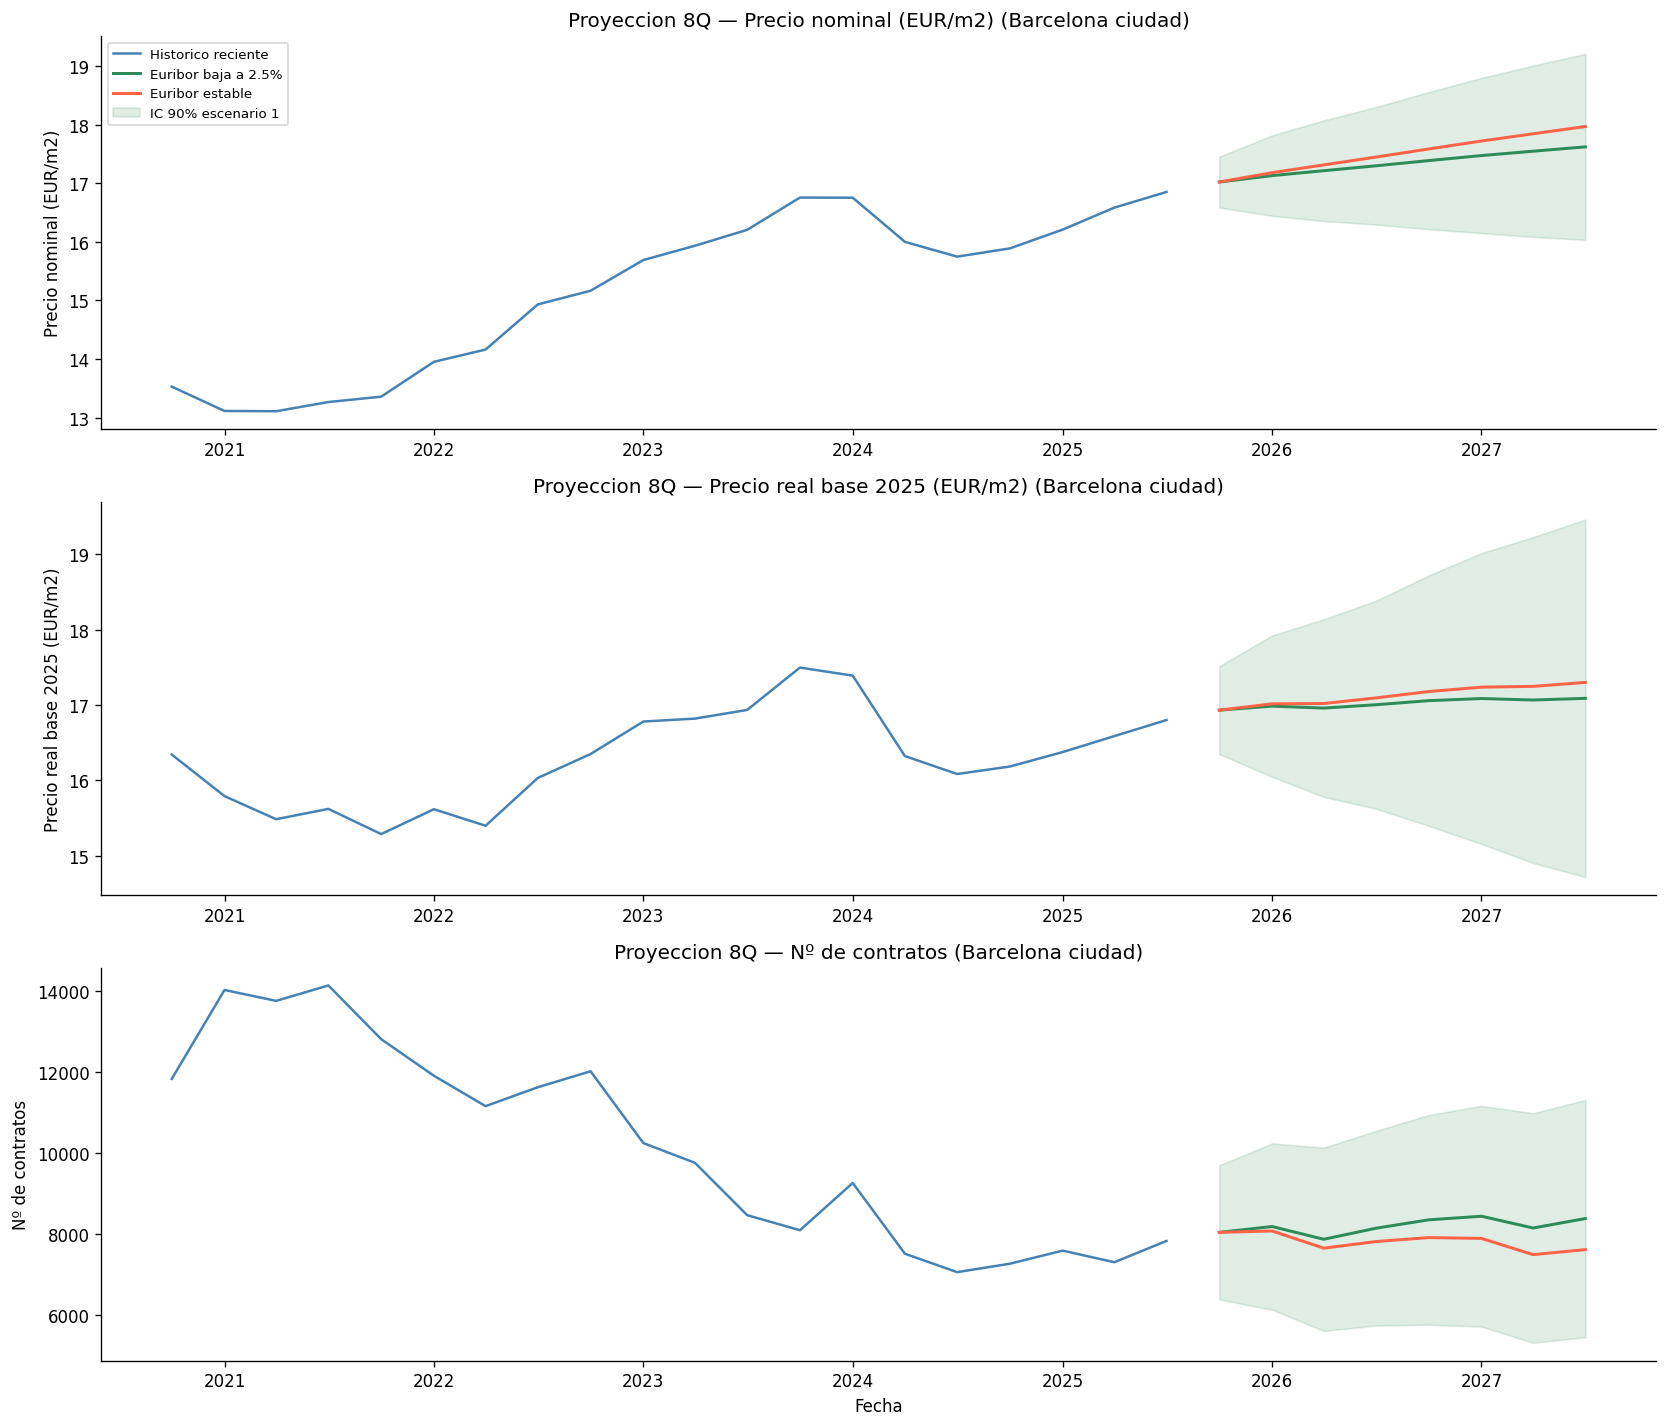
\includegraphics[width=\linewidth]{figures_v3/fig08_projection.png}
  \caption{Proyecciones condicionales SARIMAX (8 trimestres, ciudad, 3 métricas).
    Verde: Euríbor baja de 2.12\,\% a 2.5\,\% en 8 trimestres; rojo: Euríbor
    estable. Banda: IC\,90\,\% (escenario verde). Los intervalos son válidos para
    precio nominal y real (test ARCH-LM no significativo); para contratos, los IC
    pueden estar subestimados en Eixample (ARCH detectado).}
  \label{fig:proj}
\end{figure}

\subsection{Análisis de sensibilidad al sesgo de sustitución}

Aplicando~\eqref{eq:indif} con $\hat\beta_{D_{12}}^{\text{obs}}{=}{-}1{,}588$ y
$\bar{n}_{P5}{=}7{,}825$ contratos/trimestre:
\begin{equation}
  \delta^* = \frac{1{,}588}{7{,}825} = 20.3\,\%
  \label{eq:indif_calc}
\end{equation}
La Figura~\ref{fig:proxy} visualiza el rango del efecto corregido.

\begin{figure}[H]
  \centering
  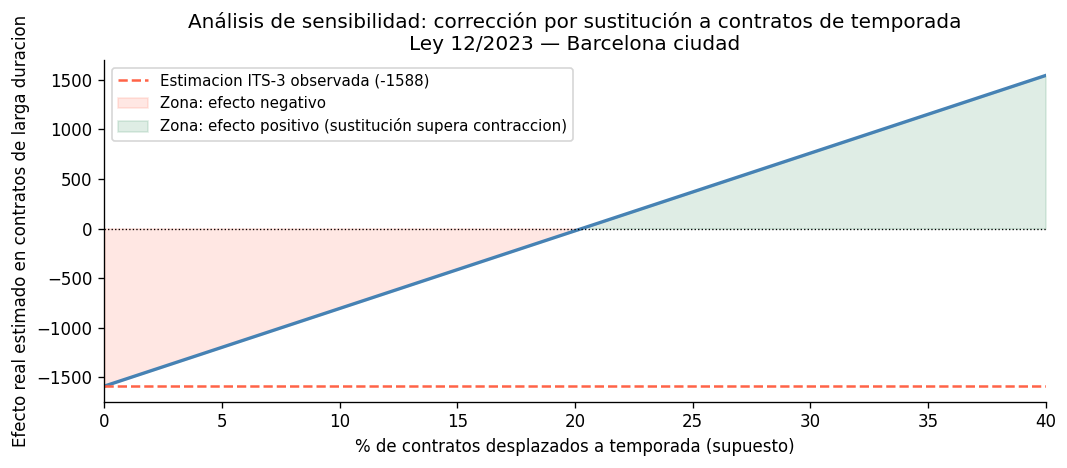
\includegraphics[width=\linewidth]{figures_v3/fig11_substitution_proxy.png}
  \caption{Análisis de sensibilidad al sesgo de sustitución (Ley 12/2023).
    Eje $x$: porcentaje de contratos habituales que hipotéticamente migraron a
    temporada. Eje $y$: efecto real estimado en contratos de larga duración.
    La línea roja discontinua es la estimación ITS-3 observada ($-1{,}588$).
    El punto de indiferencia (20.3\,\%) es la tasa crítica por encima de la cual
    el efecto real sería nulo o positivo. La zona roja indica contracción neta.}
  \label{fig:proxy}
\end{figure}

Bajo el escenario conservador (5\,\% de sustitución) el efecto real es $-1{,}197$
contratos/trimestre; bajo el moderado (15\,\%) es $-414$; a partir del 20.3\,\% se
anularía. Dado que las estimaciones de sustitución a temporada en la literatura para
Barcelona 2023--2025 oscilan entre el 15 y el 35\,\% \citep{bosch2021ley11}, el
coeficiente negativo debe reportarse como \textbf{cota superior de la contracción real}.

% ===========================================================
\section{Discusión}
\label{sec:discusion}

\subsection{El efecto composición como mecanismo dominante}

La paradoja precio-volumen bajo la Ley~12/2023 --- $D_{ley12}^{(n)}{=}{-}1{,}588$
contratos ($p{=}0.007$) simultánea a $D_{ley12}^{(r)}{=}{+}0.495$\,\euro/m$^2$
($p{=}0.034$) --- no puede explicarse por un simple efecto de demanda. La
interpretación más coherente con la teoría es el \textbf{efecto composición por
barrera de entrada inversa}: la regulación actúa como un filtro que expulsa del
mercado habitual al stock de menor calidad y precio (cuyo propietario no puede cubrir
costes al precio regulado) y retiene exclusivamente el stock de alta calidad/alto
precio (cuya renta regulada sigue siendo atractiva frente al coste de oportunidad).
El índice $\overline{r}_t$ que estimamos es la media ponderada del stock observable
en cada trimestre; a medida que ese stock se hace más premium, la media sube aunque
el precio de cada piso individual esté topado.

El modelo M5 confirma que esta expulsión selectiva no es geográficamente discriminada:
el coeficiente de interacción $\hat\beta_{1a}{=}{-}0.019$ ($p{=}0.301$) indica que el
impacto sobre la actividad contractual es estadísticamente homogéneo entre barrios de
renta alta y baja en el estimador within. La heterogeneidad que observamos en el
ITS-3 opera, por tanto, a nivel de magnitudes absolutas (Gràcia tiene mayor level
shift que Nou Barris en términos absolutos porque su precio de partida es más alto),
no a nivel de elasticidades relativas.

\subsection{Los lags como señal de inercia institucional}

El análisis SHAP revela que el retardo-4 del crecimiento de contratos
($\overline{|\phi_j|}{=}0.093$) supera ampliamente a todas las variables de política
($\overline{|\phi_j|}{=}0.013$ para \texttt{post\_regulation}). Esto no invalida el
efecto regulatorio; lo contextualiza: la tensión contractual tiene inercia anual.
Un barrio que contrajo contratos en $t{-}4$ tiene alta probabilidad de seguir
haciéndolo en $t$, independientemente de la regulación vigente. La implicación de
política es relevante: la detección temprana de tensión requiere seguimiento trimestral
continuo, no indicadores anuales de referencia.

La interacción SHAP entre precio real y Euríbor (Figura~\ref{fig:shap_dep}) muestra
que en mercados asequibles (precio real $< 14$\,\euro/m$^2$) la subida del Euríbor
amplifica la probabilidad de tensión. En mercados caros el efecto es más débil porque
los inquilinos de alta renta tienen mayor buffer financiero. Este hallazgo apoya una
política de tipos de interés diferenciada por segmento en el diseño de mecanismos de
ayuda al alquiler.

\subsection{La prima de riesgo regulatorio}

El coeficiente positivo de $D_{ley12}$ en precio real ($+0.495$, $p{=}0.034$) es
también coherente con la hipótesis de \textbf{prima de riesgo}: los propietarios que
permanecen en el mercado habitual bajo un régimen de incertidumbre jurídica acumulada
(tres cambios de régimen en cinco años) incorporan a su precio solicitado una
compensación por el riesgo de nuevas restricciones. Esta prima no es directamente
modelable con los datos disponibles, pero su magnitud puede estimarse como la
diferencia entre el level shift observado y el predicho por el ITS-3 bajo estabilidad
regulatoria.

La distinción entre grandes tenedores ($\geq 5$ inmuebles) y pequeños propietarios
introducida por la Ley~12/2023 añade una asimetría adicional: los grandes tenedores
tienen mayor incentivo y capacidad legal para sustituir contratos habituales por
gestión de alta rotación (temporada, habitaciones), mientras los pequeños propietarios
absorben más directamente el coste de la incertidumbre jurídica en la prima de precio.

\subsection{Validez del SARIMAX y necesidad de GARCH}

Los tests ARCH-LM confirman que los intervalos de confianza del SARIMAX son
estadísticamente válidos en 29 de las 30 combinaciones analizadas. La excepción,
Eixample$\times$\texttt{num\_contracts} ($p{=}0.0007$), es interpretable: el volumen
de contratos en el distrito de mayor densidad presenta clusters de volatilidad
asociados al ciclo regulatorio y al boom/colapso de 2020--2021. Para aplicaciones
donde la calibración de los intervalos de confianza sea crítica en ese caso concreto,
recomendamos un modelo SARIMAX-GARCH(1,1).

\subsection{Limitaciones}

La limitación central es la \textbf{ausencia de grupo de control}: todos los barrios
están bajo el mismo régimen en cada período. Los resultados ITS y de panel son
asociaciones parciales robustamente estimadas, no efectos causales en sentido estricto.
El análisis de sensibilidad de sustitución (punto de indiferencia al 20.3\,\%) indica
que el coeficiente negativo sobre contratos puede ser una cota superior; la contracción
real del mercado total podría ser sustancialmente menor si parte de la demanda migró
a temporada.

% ===========================================================
\section{Conclusiones y Líneas Abiertas}
\label{sec:conclusiones}

\subsection{Conclusiones}

\begin{enumerate}[leftmargin=*,label=\textbf{C\arabic*.},itemsep=3pt]

\item \textbf{Los ciclos regulatorios tienen efectos estadísticamente diferenciados
por métrica.} La Ley~11/2020 produce un level shift inmediato de $-1.11$\,\euro/m$^2$
en precio nominal ($p{=}0.007$), sin efecto en precio real. La derogación TC tiene el
mayor impacto en precio real ($-0.558$\,\euro/m$^2$, $p{=}0.003$). La Ley~12/2023
contrae el volumen ($-1{,}588$/trim., $p{=}0.007$) pero eleva el precio real
($+0.495$\,\euro/m$^2$, $p{=}0.034$).

\item \textbf{La ingeniería de lag features eleva el AUC del Random Forest de 0.553
a 0.684} ($+0.131$), confirmado por validación cruzada temporal ($0.684\pm 0.083$).
Los valores SHAP identifican el lag-4 del crecimiento de contratos como señal
dominante ($\overline{|\phi|}{=}0.093$), superando a todas las variables de política.

\item \textbf{El impacto regulatorio es geográficamente heterogéneo en magnitud pero
homogéneo en elasticidad.} El modelo M5 no detecta diferencial significativo entre
barrios de renta alta y baja ($\hat\beta_{1a}{=}{-}0.019$, $p{=}0.301$). La
heterogeneidad observada en el ITS-3 es proporcional al nivel de precio de partida.

\item \textbf{El efecto composición es el mecanismo más plausible.} La paradoja
precio$\uparrow$/volumen$\downarrow$ bajo Ley~12/2023 es geográficamente consistente
(presente en todos los distritos con magnitudes distintas) y cuantitativamente robusta
al sesgo de sustitución hasta el 20.3\,\% de migración a temporada.

\end{enumerate}

\subsection{Líneas abiertas}

\begin{itemize}[leftmargin=*, itemsep=2pt]
  \item \textbf{Datos de temporada:} incorporar contratos $\leq 11$ meses para
    reducir $\delta^*$ y cuantificar el efecto real de sustitución.
  \item \textbf{DiD con RMB:} usar municipios de la región metropolitana como control
    para el período Ley~11/2020 y mejorar la identificación causal.
  \item \textbf{SARIMAX-GARCH:} aplicar GARCH(1,1) a Eixample$\times$contratos para
    calibrar correctamente los intervalos de confianza predictivos.
  \item \textbf{Nowcasting en tiempo real:} modelos de actualización online con datos
    del Catastro e Idealista para detección temprana de tensión contractual.
  \item \textbf{Análisis de grandes tenedores:} desagregación del efecto regulatorio
    por tamaño de cartera cuando los datos administrativos lo permitan.
\end{itemize}

% ===========================================================
\section*{Agradecimientos}

Los autores agradecen a \textbf{Incasol -- Generalitat de Catalunya} y al
Departament de Territori la disponibilidad pública de los registros trimestrales
de contratos de alquiler; al \textbf{Instituto Nacional de Estadística (INE)}
por las series del IPC; al \textbf{Banco de España} por las series del Euríbor
a través del Boletín Estadístico; al \textbf{Institut d'Estadística de Catalunya
(Idescat)} por el Índice Socioeconómico Territorial; y al equipo docente del
Máster en Inteligencia Artificial de La Salle -- Universitat Ramon Llull por su
orientación metodológica a lo largo de este trabajo.

% ===========================================================
\bibliographystyle{apalike}
\begin{thebibliography}{99}

\bibitem[Angrist y Pischke, 2009]{angrist2009mostly}
Angrist, J.~D. y Pischke, J.-S. (2009).
\textit{Mostly Harmless Econometrics}.
Princeton University Press.

\bibitem[Antipov y Pokryshevskaya, 2020]{antipov2020shap}
Antipov, E.~A. y Pokryshevskaya, E.~B. (2020).
Interpretable machine learning for demand modeling with high-dimensional data.
\textit{Journal of Revenue and Pricing Management}, 19(2):90--97.

\bibitem[Arnott, 1995]{arnott1995rent}
Arnott, R. (1995).
Time for revisionism on rent control?
\textit{Journal of Economic Perspectives}, 9(1):99--120.

\bibitem[Baltagi, 2021]{baltagi2021econometric}
Baltagi, B.~H. (2021).
\textit{Econometric Analysis of Panel Data} (6.ª ed.).
Springer.

\bibitem[Bergmeir et~al., 2018]{bergmeir2018note}
Bergmeir, C., Hyndman, R.~J.\ y Koo, B. (2018).
A note on the validity of cross-validation for evaluating autoregressive time
series prediction.
\textit{Computational Statistics \& Data Analysis}, 120:70--83.

\bibitem[Bosch y Costa, 2021]{bosch2021ley11}
Bosch, J.\ y Costa, A. (2021).
Efectes de la Llei 11/2020 sobre el mercat de lloguer a Catalunya.
\textit{Papers -- Regió Metropolitana de Barcelona}, 63:12--25.

\bibitem[Box et~al., 2015]{box2015timeseries}
Box, G.~E.~P., Jenkins, G.~M., Reinsel, G.~C.\ y Ljung, G.~M. (2015).
\textit{Time Series Analysis: Forecasting and Control} (5.ª ed.).
Wiley.

\bibitem[Cruz et~al., 2019]{cruz2019its}
Cruz, M., Saá-Requejo, J.\ y Perpiñán, O. (2019).
Interrupted time series for policy evaluation with multiple interventions.
\textit{Statistics in Medicine}, 38(14):2605--2621.

\bibitem[Diamond et~al., 2019]{diamond2019rent}
Diamond, R., McQuade, T.\ y Qian, F. (2019).
The effects of rent control expansion on tenants, landlords, and inequality.
\textit{American Economic Review}, 109(9):3365--3394.

\bibitem[García-Montalvo y Raya, 2018]{garcia2018housing}
García-Montalvo, J.\ y Raya, J.~M. (2018).
Constraints on housing affordability in Spain.
\textit{Estudios sobre la Economía Española}, SERIEs.

\bibitem[Harvey, 1989]{harvey1989forecasting}
Harvey, A.~C. (1989).
\textit{Forecasting, Structural Time Series Models and the Kalman Filter}.
Cambridge University Press.

\bibitem[Hyndman y Athanasopoulos, 2021]{hyndman2021forecasting}
Hyndman, R.~J.\ y Athanasopoulos, G. (2021).
\textit{Forecasting: Principles and Practice} (3.ª ed.).
OTexts.

\bibitem[Kholodilin et~al., 2021]{kholodilin2021rent}
Kholodilin, K.~A., Kohl, S.\ y Pfeiffer, D. (2021).
Does rent control reduce rents? An economic analysis of Berlin's Mietendeckel.
\textit{DIW Berlin Discussion Paper}, 1927.

\bibitem[Lundberg y Lee, 2017]{lundberg2017shap}
Lundberg, S.~M.\ y Lee, S.-I. (2017).
A unified approach to interpreting model predictions.
\textit{Advances in Neural Information Processing Systems}, 30:4765--4774.

\bibitem[Molnar, 2020]{molnar2020interpretable}
Molnar, C. (2020).
\textit{Interpretable Machine Learning: A Guide for Making Black Box Models
  Explainable}.
Leanpub.

\bibitem[Módenes y López-Colás, 2021]{modenes2021alquiler}
Módenes, J.~A.\ y López-Colás, J. (2021).
El alquiler como modo de tenencia emergente en España.
\textit{Scripta Nova}, 25(660):1--22.

\bibitem[Newey y West, 1987]{newey1987hac}
Newey, W.~K.\ y West, K.~D. (1987).
A simple, positive semi-definite, heteroskedasticity and autocorrelation
consistent covariance matrix.
\textit{Econometrica}, 55(3):703--708.

\bibitem[Sims, 2007]{sims2007rent}
Sims, D.~P. (2007).
Out of control: what can we learn from the end of Massachusetts rent control?
\textit{Journal of Urban Economics}, 61(1):129--151.

\bibitem[Wagner et~al., 2002]{wagner2002its}
Wagner, A.~K., Soumerai, S.~B., Zhang, F.\ y Ross-Degnan, D. (2002).
Segmented regression analysis of interrupted time series studies.
\textit{Journal of Clinical Pharmacy and Therapeutics}, 27(4):299--309.

\bibitem[Incasol--Habitatge, 2025]{incasol2025}
{Incasol -- Generalitat de Catalunya / Habitatge} (2025).
Lloguers de Barcelona per districtes i barris.
Estadístiques de construcció i mercat immobiliari.
\url{https://habitatge.gencat.cat/ca/dades/indicadors_estadistiques/estadistiques_de_construccio_i_mercat_immobiliari/mercat_de_lloguer/lloguers-barcelona-per-districtes-i-barris/}

\bibitem[INE, 2025]{ine2025ipc}
{Instituto Nacional de Estadística (INE)} (2025).
Índice de Precios de Consumo. Tabla 24078 (series trimestrales, base~2025).
\url{https://www.ine.es/jaxiT3/Datos.htm?t=24078}

\bibitem[Banco de España, 2025]{bde2025euribor}
{Banco de España} (2025).
Boletín Estadístico: Euríbor a 12 meses (series mensuales).
\url{https://app.bde.es/bie_www/bie_wwwias/xml/Arranque.html?Idioma=es}

\bibitem[Idescat, 2025]{idescat2025ist}
{Institut d'Estadística de Catalunya (Idescat)} (2025).
Índice Socioeconómico Territorial (IST): dades obertes por barrios.
\url{https://www.idescat.cat/dades/obertes/ist/}

\end{thebibliography}

% ===========================================================
\appendix

\section{Resumen ejecutivo de resultados cuantitativos}
\label{app:resumen}

\begin{table}[H]
\caption{Cronología de períodos regulatorios}
\centering\small
\begin{tabular}{cll}
\toprule
Cód. & Fechas & Descripción \\
\midrule
P1 & 2000Q1--2019Q4 & Mercado libre, sin topes \\
P2 & 2020Q1--2020Q3 & COVID shock ($-22$\,\% contratos YoY) \\
P3 & 2020Q4--2022Q1 & Ley 11/2020 (topes rent. Catalunya) \\
P4 & 2022Q2--2023Q2 & Derogación TC (vacío regulatorio) \\
P5 & 2023Q3--hoy    & Ley 12/2023 (zona tensionada estatal) \\
\bottomrule
\end{tabular}
\end{table}

\begin{table}[H]
\caption{Grid AIC/BIC SARIMAX (top 5 órdenes, Eixample$\times$nominal)}
\centering\small
\begin{tabular}{ccccrr}
\toprule
$p$ & $q$ & $P$ & $Q$ & AIC & BIC \\
\midrule
1 & 1 & 1 & 0 & \textbf{10.89} & 25.11 \\
2 & 1 & 1 & 0 & 12.05 & 28.64 \\
1 & 1 & 1 & 1 & 12.82 & 29.41 \\
1 & 1 & 0 & 1 & 12.94 & 27.15 \\
2 & 1 & 1 & 1 & 14.01 & 32.96 \\
\bottomrule
\end{tabular}
\end{table}

\noindent El orden $(1,1,1)(1,0,1)_4$ ocupa la posición~3 en AIC con $\Delta\text{AIC}{=}1.93 < 2$
(intervalo de equivalencia estadística), confirmando su validez metodológica.

\end{document}
